\newcommand{\figureplaceholder}[2][0.9\textwidth]{%
	\fbox{%
		\begin{minipage}[c][6cm][c]{#1}
			\centering
			\textcolor{gray}{\large #2}
		\end{minipage}%
	}%
}
\chapter{Experiments}
\label{chapt::Experiments}
%
%This chapter presents the experiments. It is a crucial part of the thesis and has to dominate in the thesis. 
%The experiments and their analysis should be done in the way commonly accepted in the scientific community (eg. benchmark datasets, cross validation of elaborated results, reproducibility and replicability of tests etc).
%
%
This chapter presents the configuration process and the results of experiments conducted in the test environment. The main objective of the research was to empirically verify the effectiveness and assess the stability of RL agents. The following sections discuss in detail used hyperparameters, the experiments conducted, and analyze the results obtained in the context of the research objectives.
\section{Methodology}
This chapter outlines the research framework, training methods employed and training configuration used throughout the study. It also outlines the evaluation procedure and performance metrics employed to ensure fair and consistent comparisons between the approaches under investigation.
\subsection{Research Framework}

The experimental study focuses on comparing two reinforcement learning configurations within a level-limited Curriculum Learning environment: a baseline PPO agent and a PPO agent supported by Generative Adversarial Imitation Learning. The objective is not to train an agent capable of completing the entire Rummikub curriculum, but to evaluate how effectively both approaches acquire the sequence of skills represented by the selected curriculum level, which are described in \ref{tab:CL_seg}.
The experiments are intended to determine whether the addition of GAIL improves the learning process compared with the PPO baseline. In particular, the study investigates whether demonstration-based guidance allows the agent to reach curriculum milestones using fewer training steps, reduces variability between independent runs, and produces a more stable learning curve.

The first stage involved preliminary training experiments in the complete game environment. No meaningful learning progress was observed. Due to the highly sparse reward structure of the complete Rummikub environment, the agent was unable to discover effective strategies through exploration alone. Consequently, repeating the same training procedure using multiple independent runs did not provide statistically meaningful results. Therefore, the complete game environment was excluded from the experiment in this thesis, and the statistical analysis focused exclusively on training an agent that can effectively generate basic sequences on the board based on the presence of another sequence.

%The second stage involved the development of a curriculum learning environment, in which the original game was divided into a series of increasingly challenging training stages.  The environment was designed to mitigate the sparse reward problem by introducing game mechanics incrementally, allowing the agent to acquire elementary skills before progressing to more complex tasks.
%Based on preliminary experiments and analysis of skills introduced at successive curriculum stages, Level 11 was selected as the target evaluation level. At this stage, the agent must independently place a complete three-tile sequence while another is already present on the board. Consequently, this task assesses the agent's ability to perform a complete tile-placement procedure in a state containing additional, task-irrelevant board elements. Reaching and completing this level was adopted as a consistent intermediate learning milestone for comparing the training efficiency of the evaluated methods. The target was considered to have been achieved when the agent successfully completed level 11 and advanced to level 12.

 Two agent configurations were trained using the Proximal Policy Optimization (PPO) algorithm. Each configuration underwent multiple independent training runs with identical hyperparameter settings and the same ML-Agents seed, ensuring consistent training conditions. While the training configuration remained fixed, as shown in tables \ref{tab:ppo_hyperparameters}, \ref{tab:auxiliary}, the Unity environment continued to generate random game states, providing different learning experiences across training runs.

Finally, the trained models were evaluated under identical evaluation conditions. The evaluation consisted of two stages. First, the ability of each training run to finish the 11th curriculum level was analyzed. Second, the trained policies were assessed in a separate evaluation procedure by executing multiple independent episodes on the 11th curriculum level and measuring the percentage of successfully completed episodes. The obtained results were subsequently analyzed to compare the effectiveness, robustness, and learning stability of the investigated training configurations. The baseline PPO model was then compared with an enhanced PPO model using Generative Adversarial Imitation Learning (GAIL).


\subsection{Training methods}

This experimental study compares the performance of several training configurations based on the PPO algorithm. In addition to the baseline implementation, selected learning support technique was incorporated to investigate their impact on the agent's learning performance. The sections \ref{Enhancement_tech_1}, \ref{Enhancement_tech_2}, \ref{Enhancement_tech_3} present the theoretical background and implementation details of techniques,
The following training configurations were evaluated:
\begin{itemize}
	\item PPO which is baseline RL algorithm in ML-Agents, used as reference method.
	\item PPO + GAIL - combined with GAIL using expert demonstrations.
\end{itemize}
The baseline PPO agent was used as the reference model, and the other configuration examined the contribution of individual learning support technique to overall training performance.
%jakie metody są porównywane
%\subsection{Training configuration and hyperparameters}
%yaml configurations

All training configurations used the same neural network architecture and hyperparameter settings. This ensured that any performance differences observed during the experiments were primarily due to the learning support techniques applied, rather than variations in the training configuration.
\begin{table}[H]
	\centering
	\caption{PPO hyperparameters and neural network architecture used in all training configurations.}
	\label{tab:ppo_hyperparameters}
	\begin{tabular}{ll}
		\toprule
		\textbf{Parameter} & \textbf{Value} \\
		\midrule
		Trainer & PPO \\
		Batch size & 512 \\
		Buffer size & 8192 \\
		Learning rate & $3 \times 10^{-4}$ \\
		Learning rate schedule & Linear \\
		Beta & 0.001 \\
		Epsilon & 0.15 \\
		Lambda & 0.95 \\
		Number of epochs & 3 \\
		Discount factor ($\gamma$) & 0.995 \\
		Reward strength & 1.0 \\
		Time horizon & 256 \\
		Maximum training steps & 2,000,000 \\
		seed & 42\\
		\midrule
		Observation normalization & Enabled \\
		Hidden units & 128 \\
		Hidden layers & 2 \\
		Memory type & LSTM \\
		Memory size & 128 \\
		Sequence length & 32 \\
		\midrule
		Number of lessons & 12 \\
		Performance measure & Reward \\
		Promotion threshold & 0.7 \\
		Minimum lesson length & 500 episodes \\
		Signal smoothing & Enabled \\
		Require environment reset & Disabled \\
		
		\bottomrule
	\end{tabular}
\end{table}
Each agent was trained independently using identical environment settings and the same maximum number of training steps. The baseline PPO configuration served as the reference setup, while the remaining configurations extended the baseline with selected auxiliary learning technique. Hyperparameters specific to Generative Adversarial Imitation Learning were enabled only for the corresponding training configurations, whereas all other PPO parameters remained unchanged.

Table \ref{tab:ppo_hyperparameters} summarizes the PPO hyperparameters shared across all training configurations, the neural network architecture used in the experiments and the curriculum learning configuration, including the lesson progression criteria.
Additional hyperparameters associated with auxiliary learning technique listed in the Table \ref{tab:auxiliary}.
\begin{table}[H]
	\centering
	\caption{Hyperparameters of the auxiliary learning techniques.}
	\label{tab:auxiliary}
	\begin{tabular}{lll}
		\toprule
		\textbf{Module} & \textbf{Parameter} & \textbf{Value} \\
		\midrule
		\multirow{5}{*}{GAIL}
		& Strength & 0.4 \\
		& Learning rate & $1\times10^{-4}$ \\
		& Discount factor ($\gamma$) & 0.99 \\
		& Use VAIL & False \\
		& Use actions & True \\
		\bottomrule
	\end{tabular}
\end{table}

\subsubsection{Hardware}
This section presents the physical components of device under which the experiment was conducted. 
\begin{itemize}
	\item CPU - AMD Ryzen 9 7940HS with Radeon 780M Graphics, 4.00 GHz
	\item GPU - NVIDIA GeForce RTX 4050 and AMD Radeon 280M
	\item 16.0 GB of RAM
	\item 64-bit Windows 11
\end{itemize}
%
%\begin{itemize}
%\item description of methodology of experiments
%\item description of experimental framework (description of user interface of research applications – move to an appendix)
%\end{itemize}
%
%
%\section{Data sets}
%
%\begin{itemize}
%\item description of data sets
%\end{itemize}
%
%
\subsection{Evaluation methods}
The evaluation procedure was divided into two complementary stages. The first stage involved analyzing the training process and how individual agents progressed through the Curriculum Learning environment. The second stage involved a post-training evaluation conducted at a fixed curriculum level. This approach enabled both the efficiency of the learning process and the final performance of the trained policies to be assessed.


Following the training stage, each trained neural network was evaluated independently at the 11th curriculum level. During this evaluation, the NN operated in inference mode, with no updates to its parameters. Each network underwent testing for 1,000 episodes in identical curriculum learning level. Since ten models were evaluated for each method, there were 10,000 episodes for PPO and 10,000 for PPO with GAIL, making 20,000 in total.



\section{Results}
This section will present and analyzes the results of experiments, comparing them across different settings.
\subsection{Baseline}
This section presents the results of the baseline model during training, as well as the final evaluation results of the baseline model.
\subsubsection{Learning results}
The figure \ref{fig:ppo_curriculum_CumulativeReward} presents a graph \textbf{Cumulative Rewards} \ref{Env::metrics}, obtained during the training process of ten basic independent PPO baseline agents. At the beginning of training, nearly every agent achieved scores ranging from $-3.9$ to $-3.6$. During the first 100,000 to 200,000 steps, the environmental reward suddenly increased to 0 and positive values, which may indicate the simplicity of the first levels. 

In the subsequent stages, most training runs followed a repeated pattern of gradual reward improvement followed by a sudden decrease. These decreases were most likely associated with transitions to more difficult curriculum levels. After entering a new level, the agents initially obtained lower rewards and subsequently adapted their policies to the new task. Nevertheless, several decreases below $-2$ indicate that some curriculum stages introduced a considerable increase in difficulty.



\begin{figure}[H]
	\centering
	
	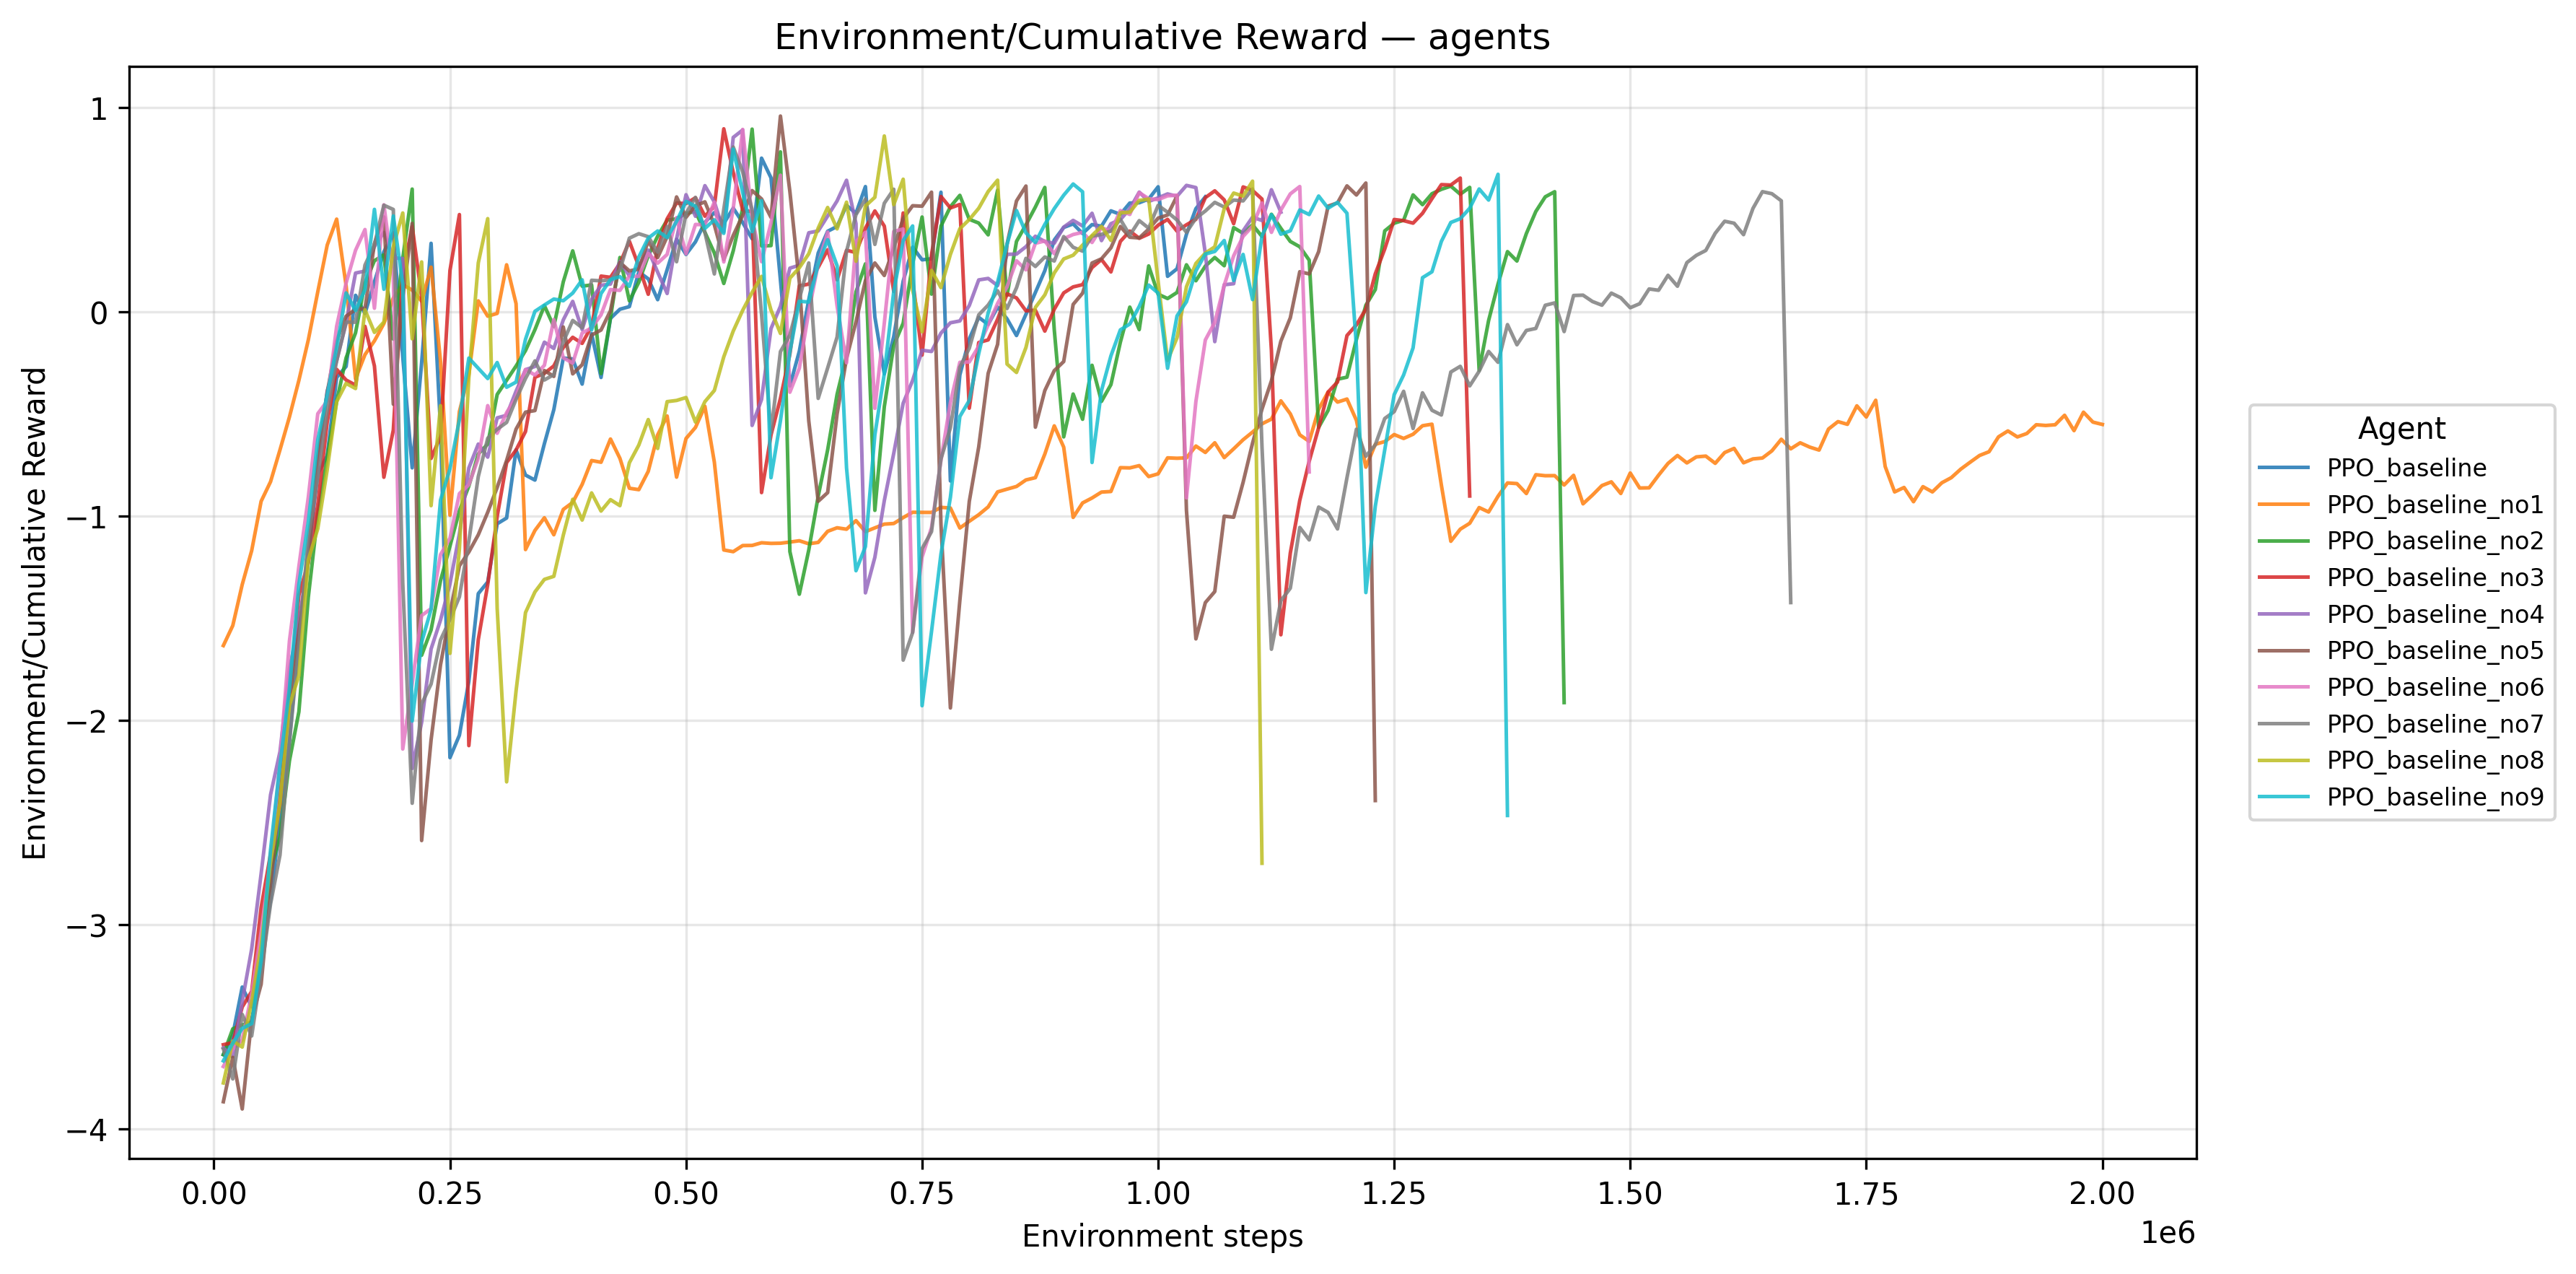
\includegraphics[width=1.0\textwidth]{images/baseline_results/Environment_Cumulative_Reward_agents.png}
	%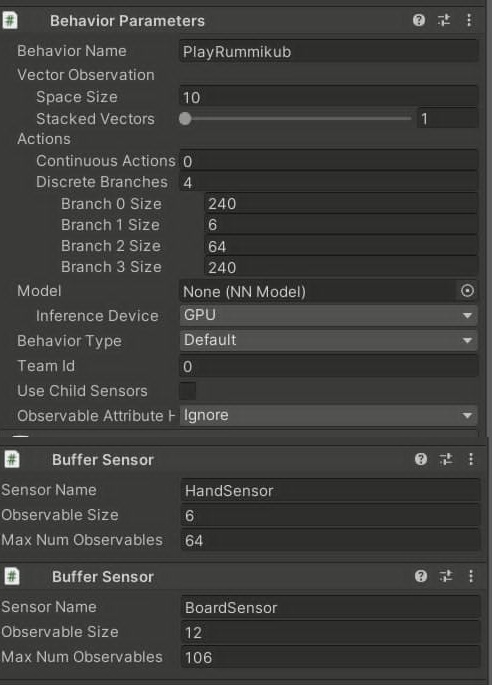
\includegraphics[width=0.7\textwidth]{images/BF_image.jpg}
	\caption{
	Cumulative reward graph of 10 baseline agents
	}
	\label{fig:ppo_curriculum_CumulativeReward}
\end{figure}
While most agents exhibited similar general learning patterns, differences were observed in the number of steps required to recover after a level transition. The most distinct result was obtained by the \textit{PPO\_baseline\_no1} agent. Its reward reached positive values during the early stage of training but subsequently remained below zero for most of the recorded process. Although this agent achieved positive rewards earlier than the remaining agents, its rapid initial improvement did not translate into successful progression to the predefined target level. This indicates that the agent encountered difficulties in adapting to one of the subsequent curriculum tasks within the available training budget. 
The \textit{PPO\_baseline\_no7} agent required substantially more training steps than most of the other agents, however, it did reach the target level.  
\begin{figure}[H]
	\centering
	
	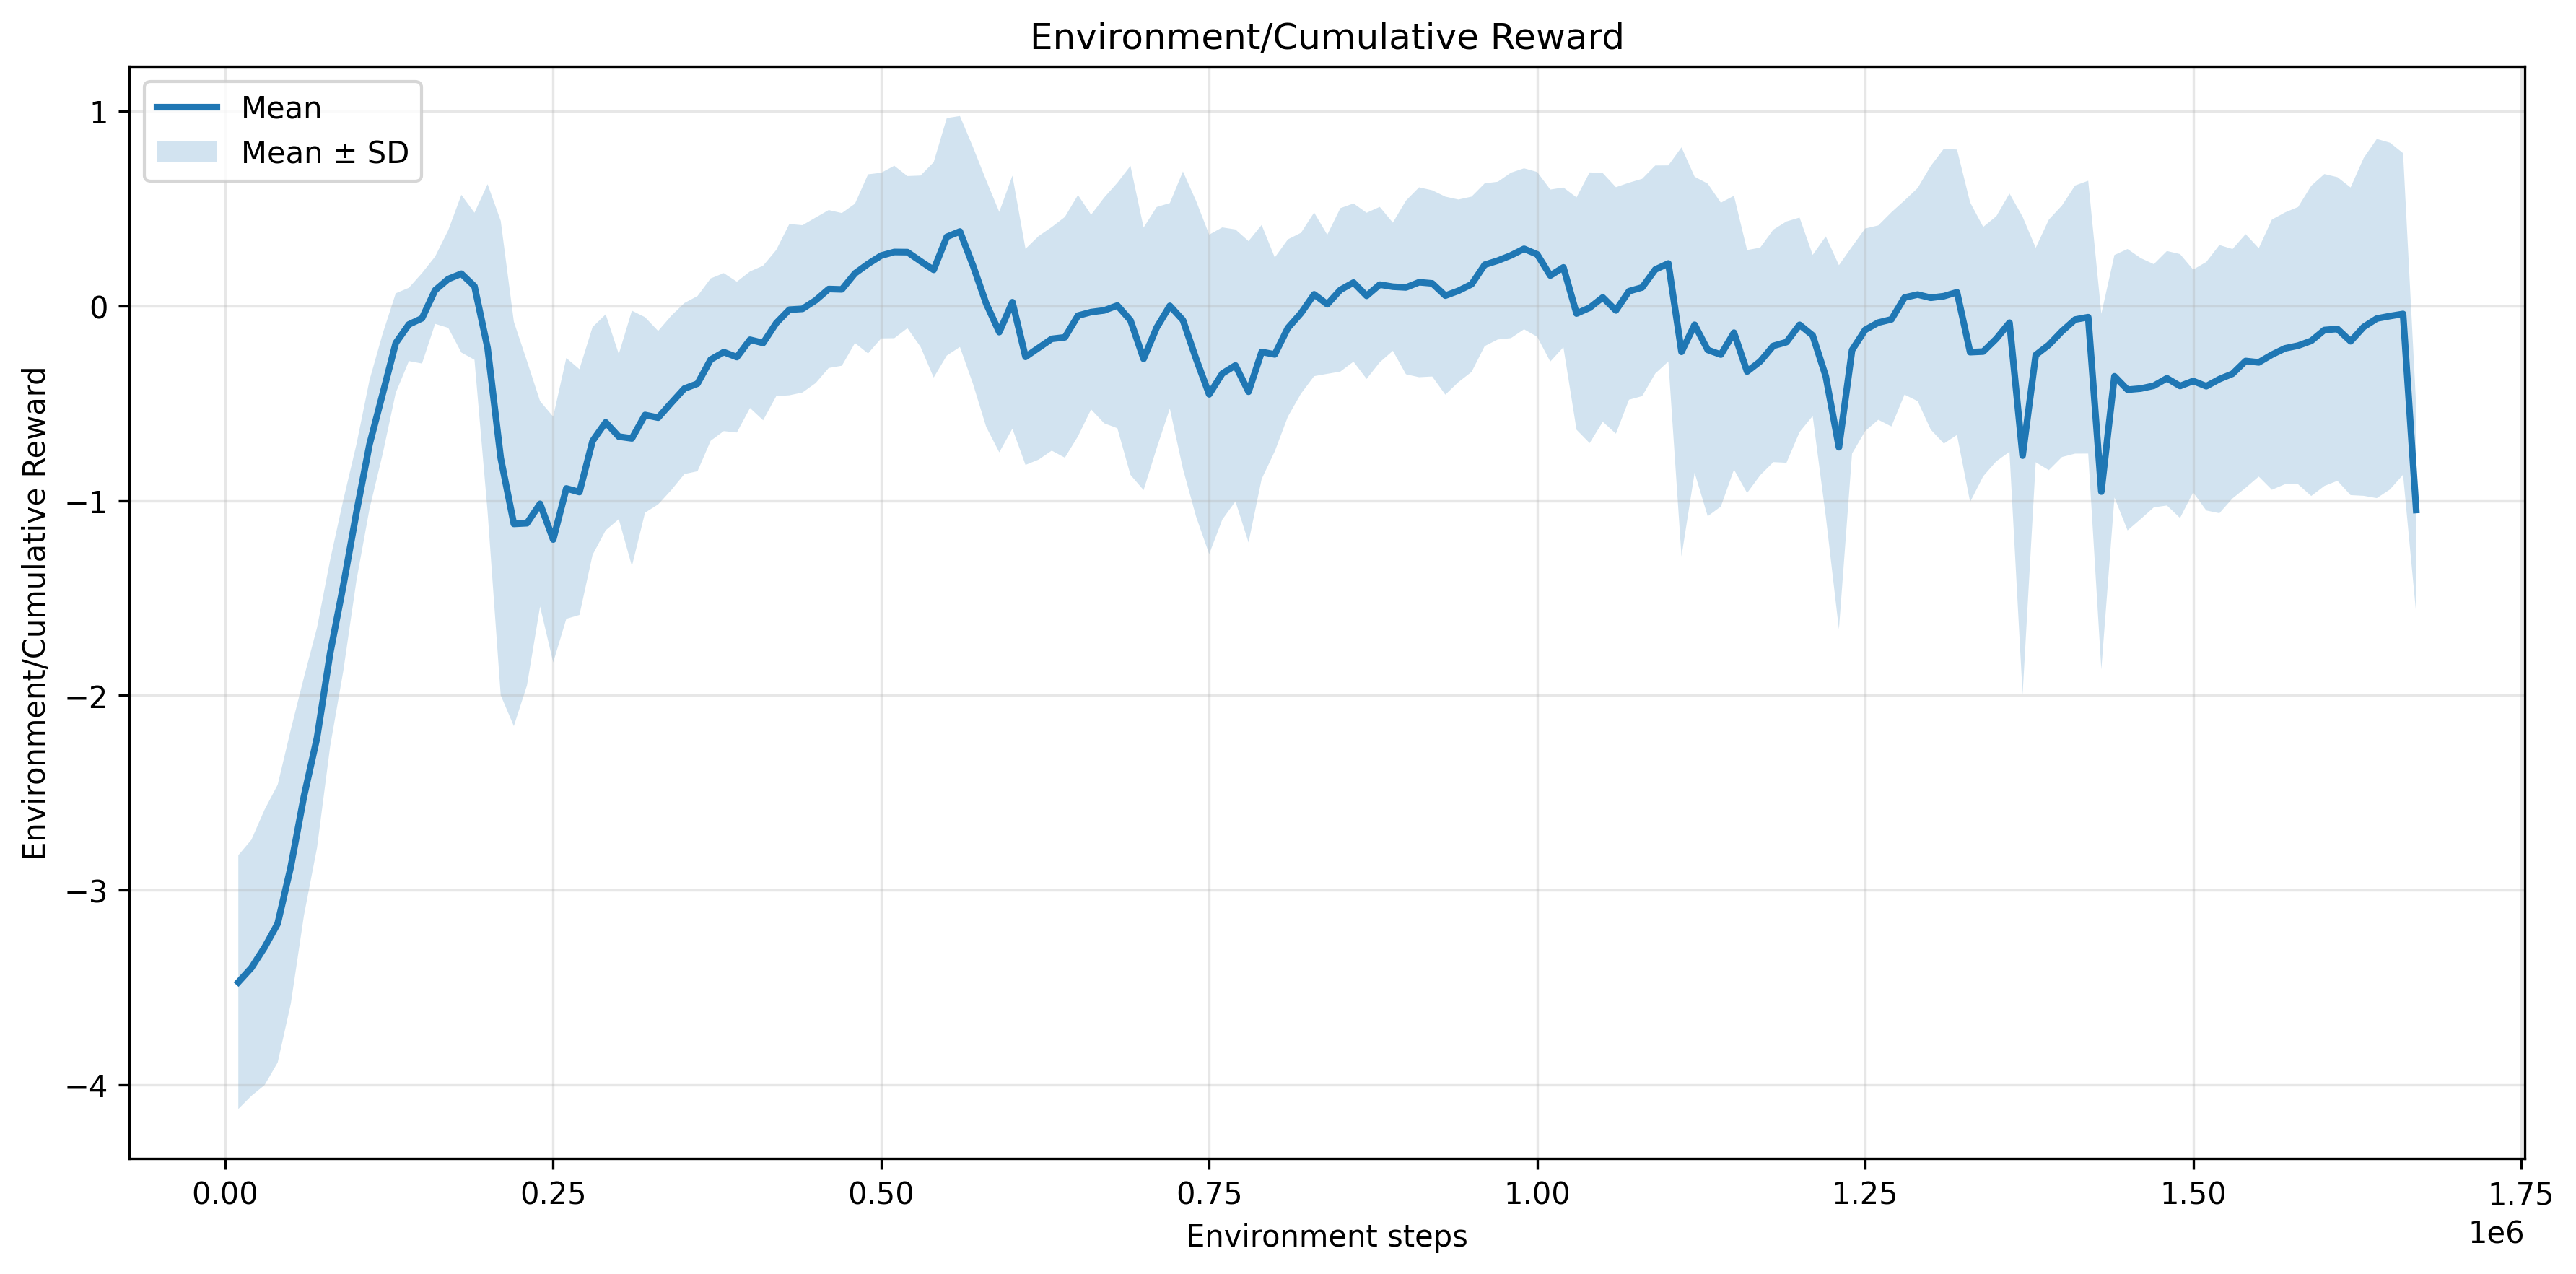
\includegraphics[width=1.0\textwidth]{images/baseline_results/Environment_Cumulative_Reward_mean_sd.png}
	%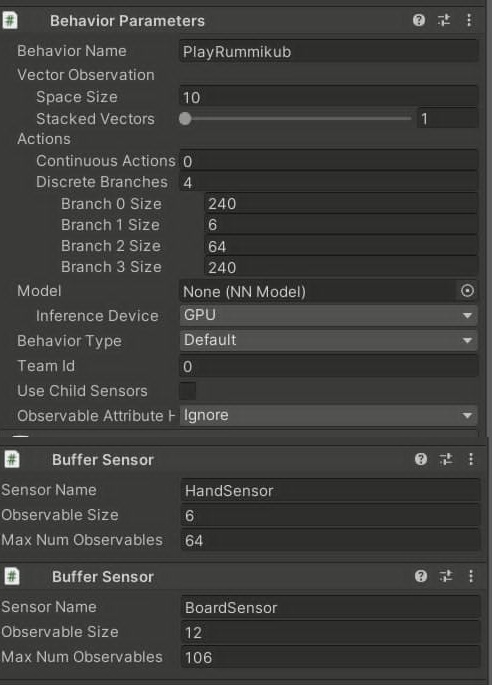
\includegraphics[width=0.7\textwidth]{images/BF_image.jpg}
	\caption{
		Cumulative reward mean and SD graph of 10 baseline agents
	}
	\label{fig:ppo_curriculum_CumulativeReward_mean_STD}
\end{figure}
Figure \ref{fig:ppo_curriculum_CumulativeReward_mean_STD} summarizes the cumulative rewards obtained by the PPO Baseline agents. The mean reward increased rapidly from approximately $-3.5$ at the beginning of training and reached values close to zero within the first 200,000 environment steps. This confirms that the agents generally acquired the initial curriculum skills relatively quickly. The subsequent fluctuations around zero reflect the repeated process of adapting to increasingly difficult tasks rather than a continuous improvement within a single unchanged environment.

The standard-deviation band becomes wider as training progresses, indicating increasing differences in the learning progress of individual agents. This variation results partly from agents reaching successive curriculum levels at different times and therefore performing tasks of different difficulty at the same training step. Consequently, the averaged curve describes the general learning tendency of the PPO Baseline group, whereas the wide standard deviation shows that the speed of acquiring more complex skills was not uniform across training runs.

The figure \ref{fig:ppo_baseline_lessonNumber} illustrates the progression of ten independently trained agents through the curriculum using the PPO baseline configuration. The stepwise shape of the curves is a consequence of the structure of curriculum learning, whereby an agent remains at a given level until the necessary promotion criteria have been met.

\begin{figure}[H]
	\centering
	
	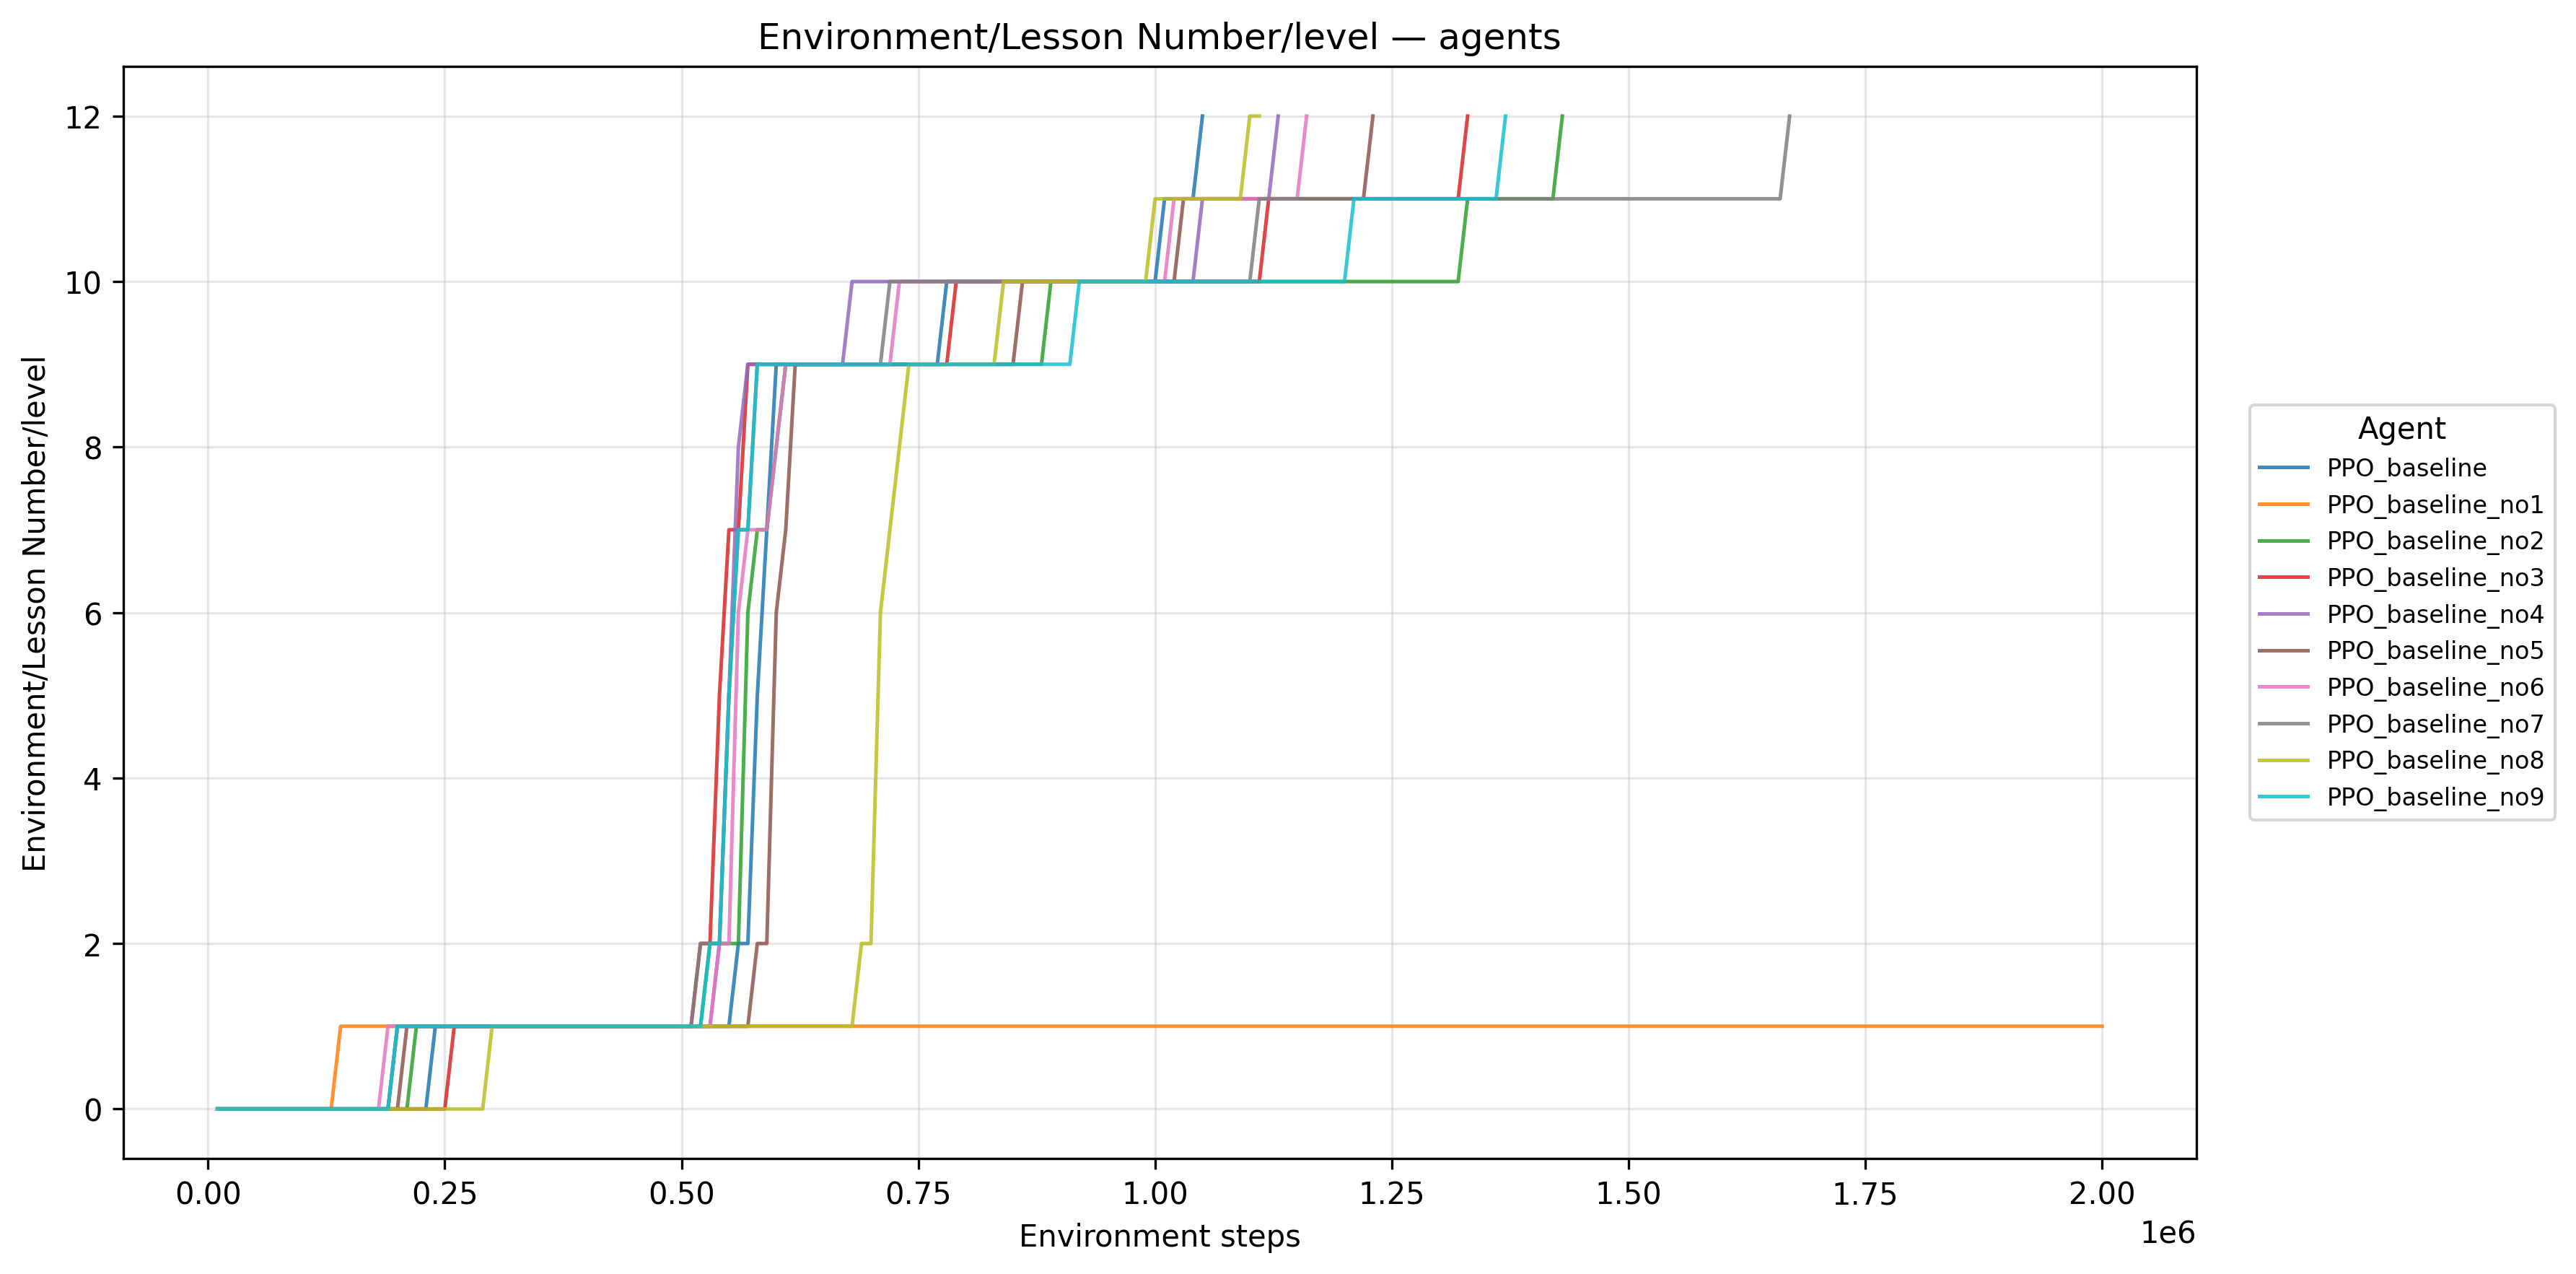
\includegraphics[width=1.0\textwidth]{images/baseline_results/Environment_Lesson_Number_level_agents.png}
	%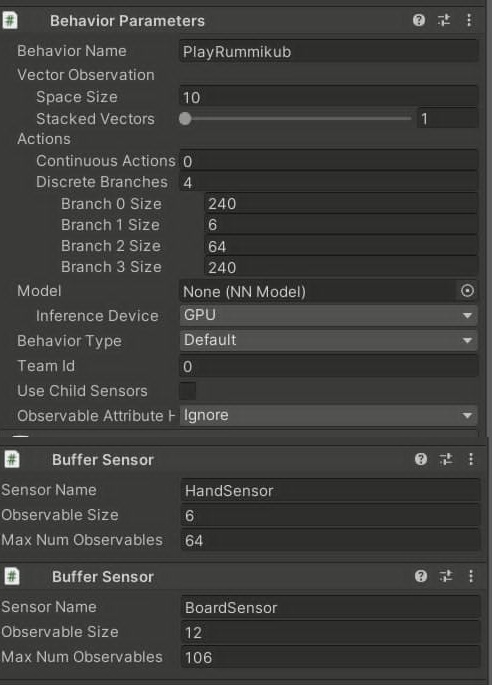
\includegraphics[width=0.7\textwidth]{images/BF_image.jpg}
	\caption{
		Curriculum progression of individual 10 baseline agents
	}
	\label{fig:ppo_baseline_lessonNumber}
\end{figure}
Most agents completed the initial curriculum level after approximately 200,000--300,000 environment steps. The exception was the \textit{PPO\_baseline\_no1} agent, which advanced to level 1 earlier, after approximately 140,000 steps. However, it remained at this level until the end of its training process at 2 million steps. Consequently, this agent did not reach the predefined target. This observation also explains why its curriculum reward remained predominantly negative in the later part of the training process, the agent was unable to satisfy the promotion criterion for level 1.

The remaining nine agents successfully progressed beyond the initial stages of the curriculum. Most of them remained at Level 1 until they had taken approximately 500,000--600,000 steps, after which they advanced rapidly through Levels 2–9. The short amount of time spent at several of these intermediate levels suggests that they found the tasks associated with these levels easier than those associated with the longer plateaus. However, the exact transition steps should be interpreted as approximate, as the metric was recorded at fixed summary intervals.

Significant differences between the agents emerged at levels 9, 10 and 11. Several agents remained at level 9 for a long time before being promoted to level 10. The time taken to advance beyond level 10 also varied considerably, with some agents achieving this in approximately 1 million steps, while others required more than 1.3 million. These plateaus suggest that the later curriculum tasks were more challenging and required more experience to meet the promotion criterion.

The \textit{PPO\_baseline\_no7} agent required the largest number of environment steps among the successful training runs. It remained at level 11 for an extended period and reached the final target only after approximately 1.6 million steps. By contrast, the fastest agents reached the same stage after approximately 1.1 million steps. Overall, nine out of ten agents reached the target, but their progression rates differed considerably despite the use of the same training configuration.

\begin{figure}[H]
	\centering
	
	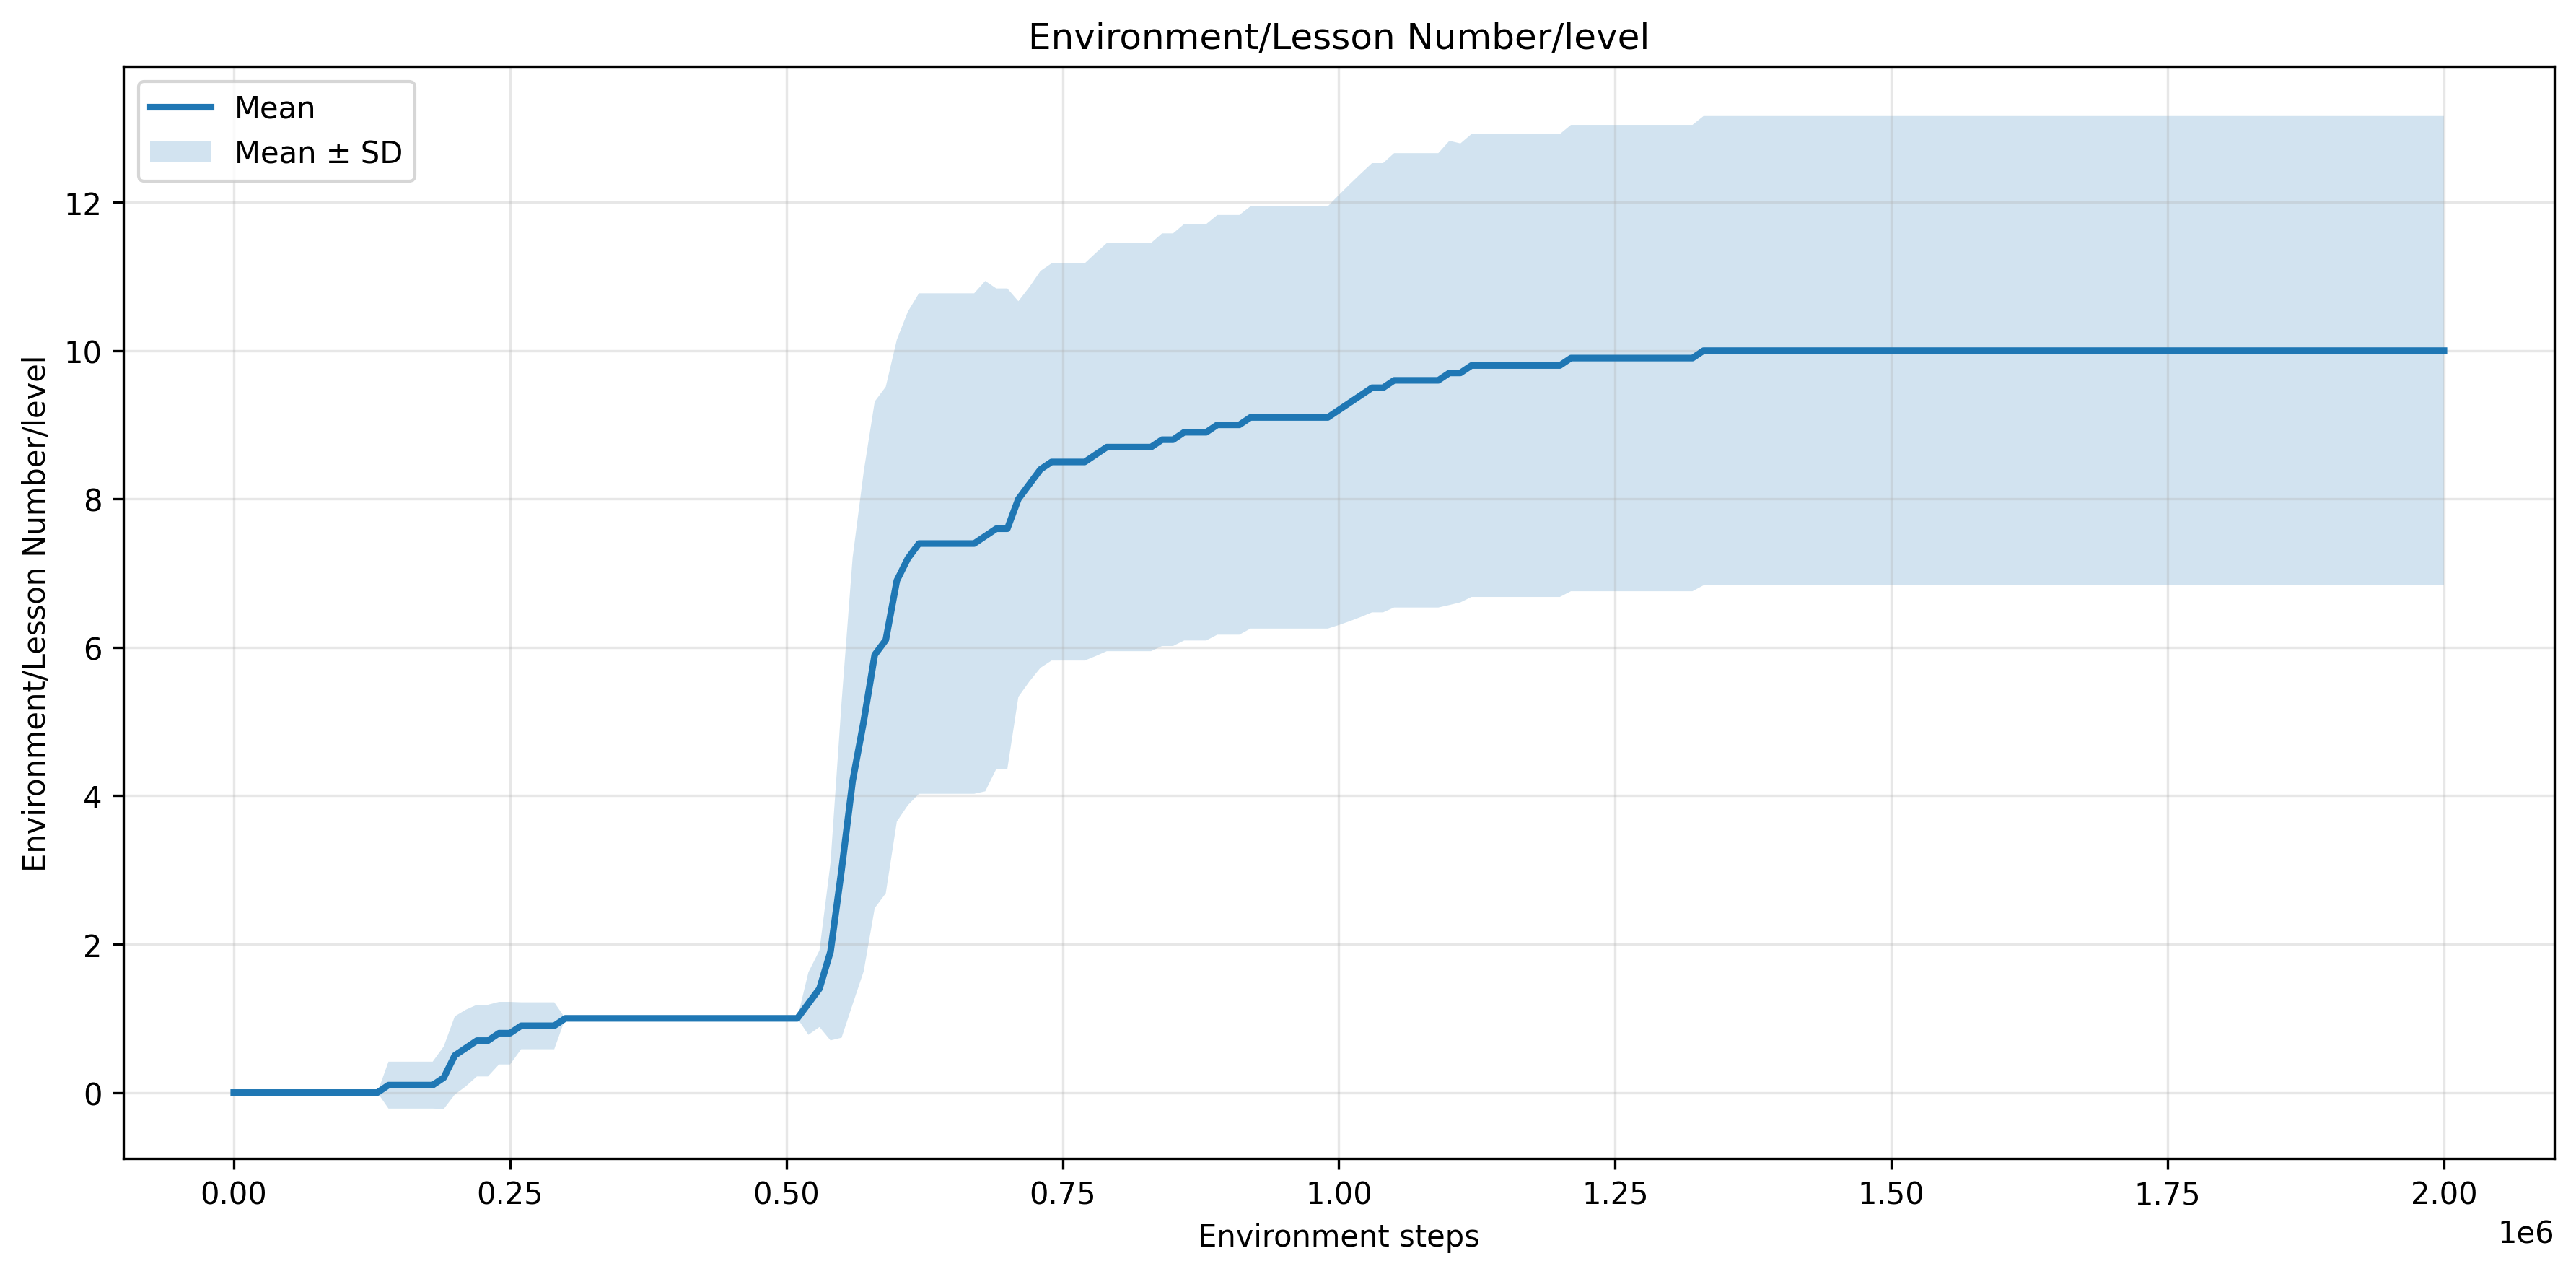
\includegraphics[width=1.0\textwidth]{images/baseline_results/Environment_Lesson_Number_level_mean_sd.png}
	%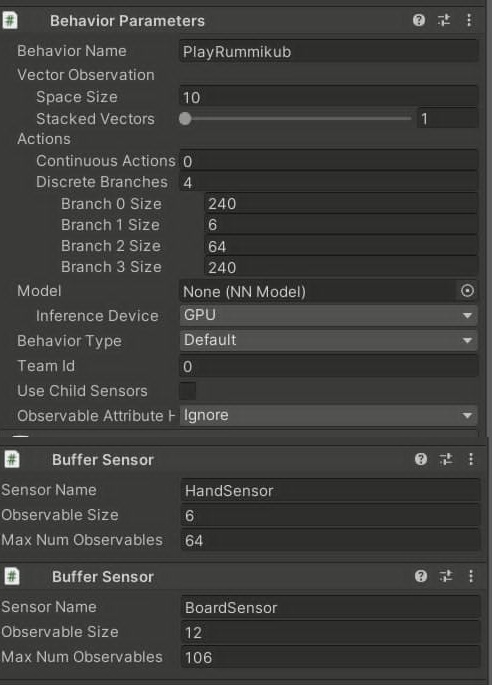
\includegraphics[width=0.7\textwidth]{images/BF_image.jpg}
	\caption{
		Curriculum progression mean and SD of individual 10 baseline agents
	}
	\label{fig:ppo_baseline_lessonNumber_mean_SD}
\end{figure}

Figure \ref{fig:ppo_baseline_lessonNumber_mean_SD} summarizes the curriculum progress of the PPO Baseline agents. The mean lesson number increased rapidly after approximately 500,000 environment steps, confirming that most agents progressed through several intermediate tasks within a relatively short training interval. The subsequent slower increase indicates that the later curriculum tasks required more experience and produced greater differences in progression speed.

The widening standard-deviation band reflects the increasing separation between agents that reached the target and the single agent that remained at an early curriculum level and failed to complete the training objective. The decrease in the mean observed in the later part of the graph does not represent a regression of the trained policies. Instead, agents that reached the target stopped producing further observations, leaving the unsuccessful and slower runs with a progressively greater influence on the calculated statistics. Therefore, the final section of the curve is based on a changing and decreasing number of active runs and should not be interpreted as the mean progress of all ten agents.

The figure \ref{fig:ppo_baseline_entropy} demonstrate changes in policy entropy value \ref{Env::metrics} during the training agents using the PPO baseline configuration. 
At the beginning of training, most agents exhibited an entropy value of approximately 5.9. During the first 500,000 environment steps, entropy gradually decreased to approximately 2.4--2.6. This general downward trend indicates that the agents progressively reduced random exploration as they acquired more consistent action-selection strategies for the initial curriculum tasks.

Most agents experienced a substantial increase in entropy between approximately 550,000 and 700,000 steps. According to the curriculum level progression shown in \ref{fig:ppo_baseline_lessonNumber}, this interval corresponded to rapid advancement through several successive levels of the curriculum. Therefore, the increase in entropy suggests that the agents began to explore a wider range of actions after encountering new tasks and changing environmental conditions. After this period, entropy generally stabilized between 3.3 and 3.9, although temporary fluctuations remained visible. Many of these fluctuations coincided with progression to subsequent curriculum levels and may reflect the need to adapt the learned policy to the requirements of new tasks.

\begin{figure}[H]
	\centering
	
	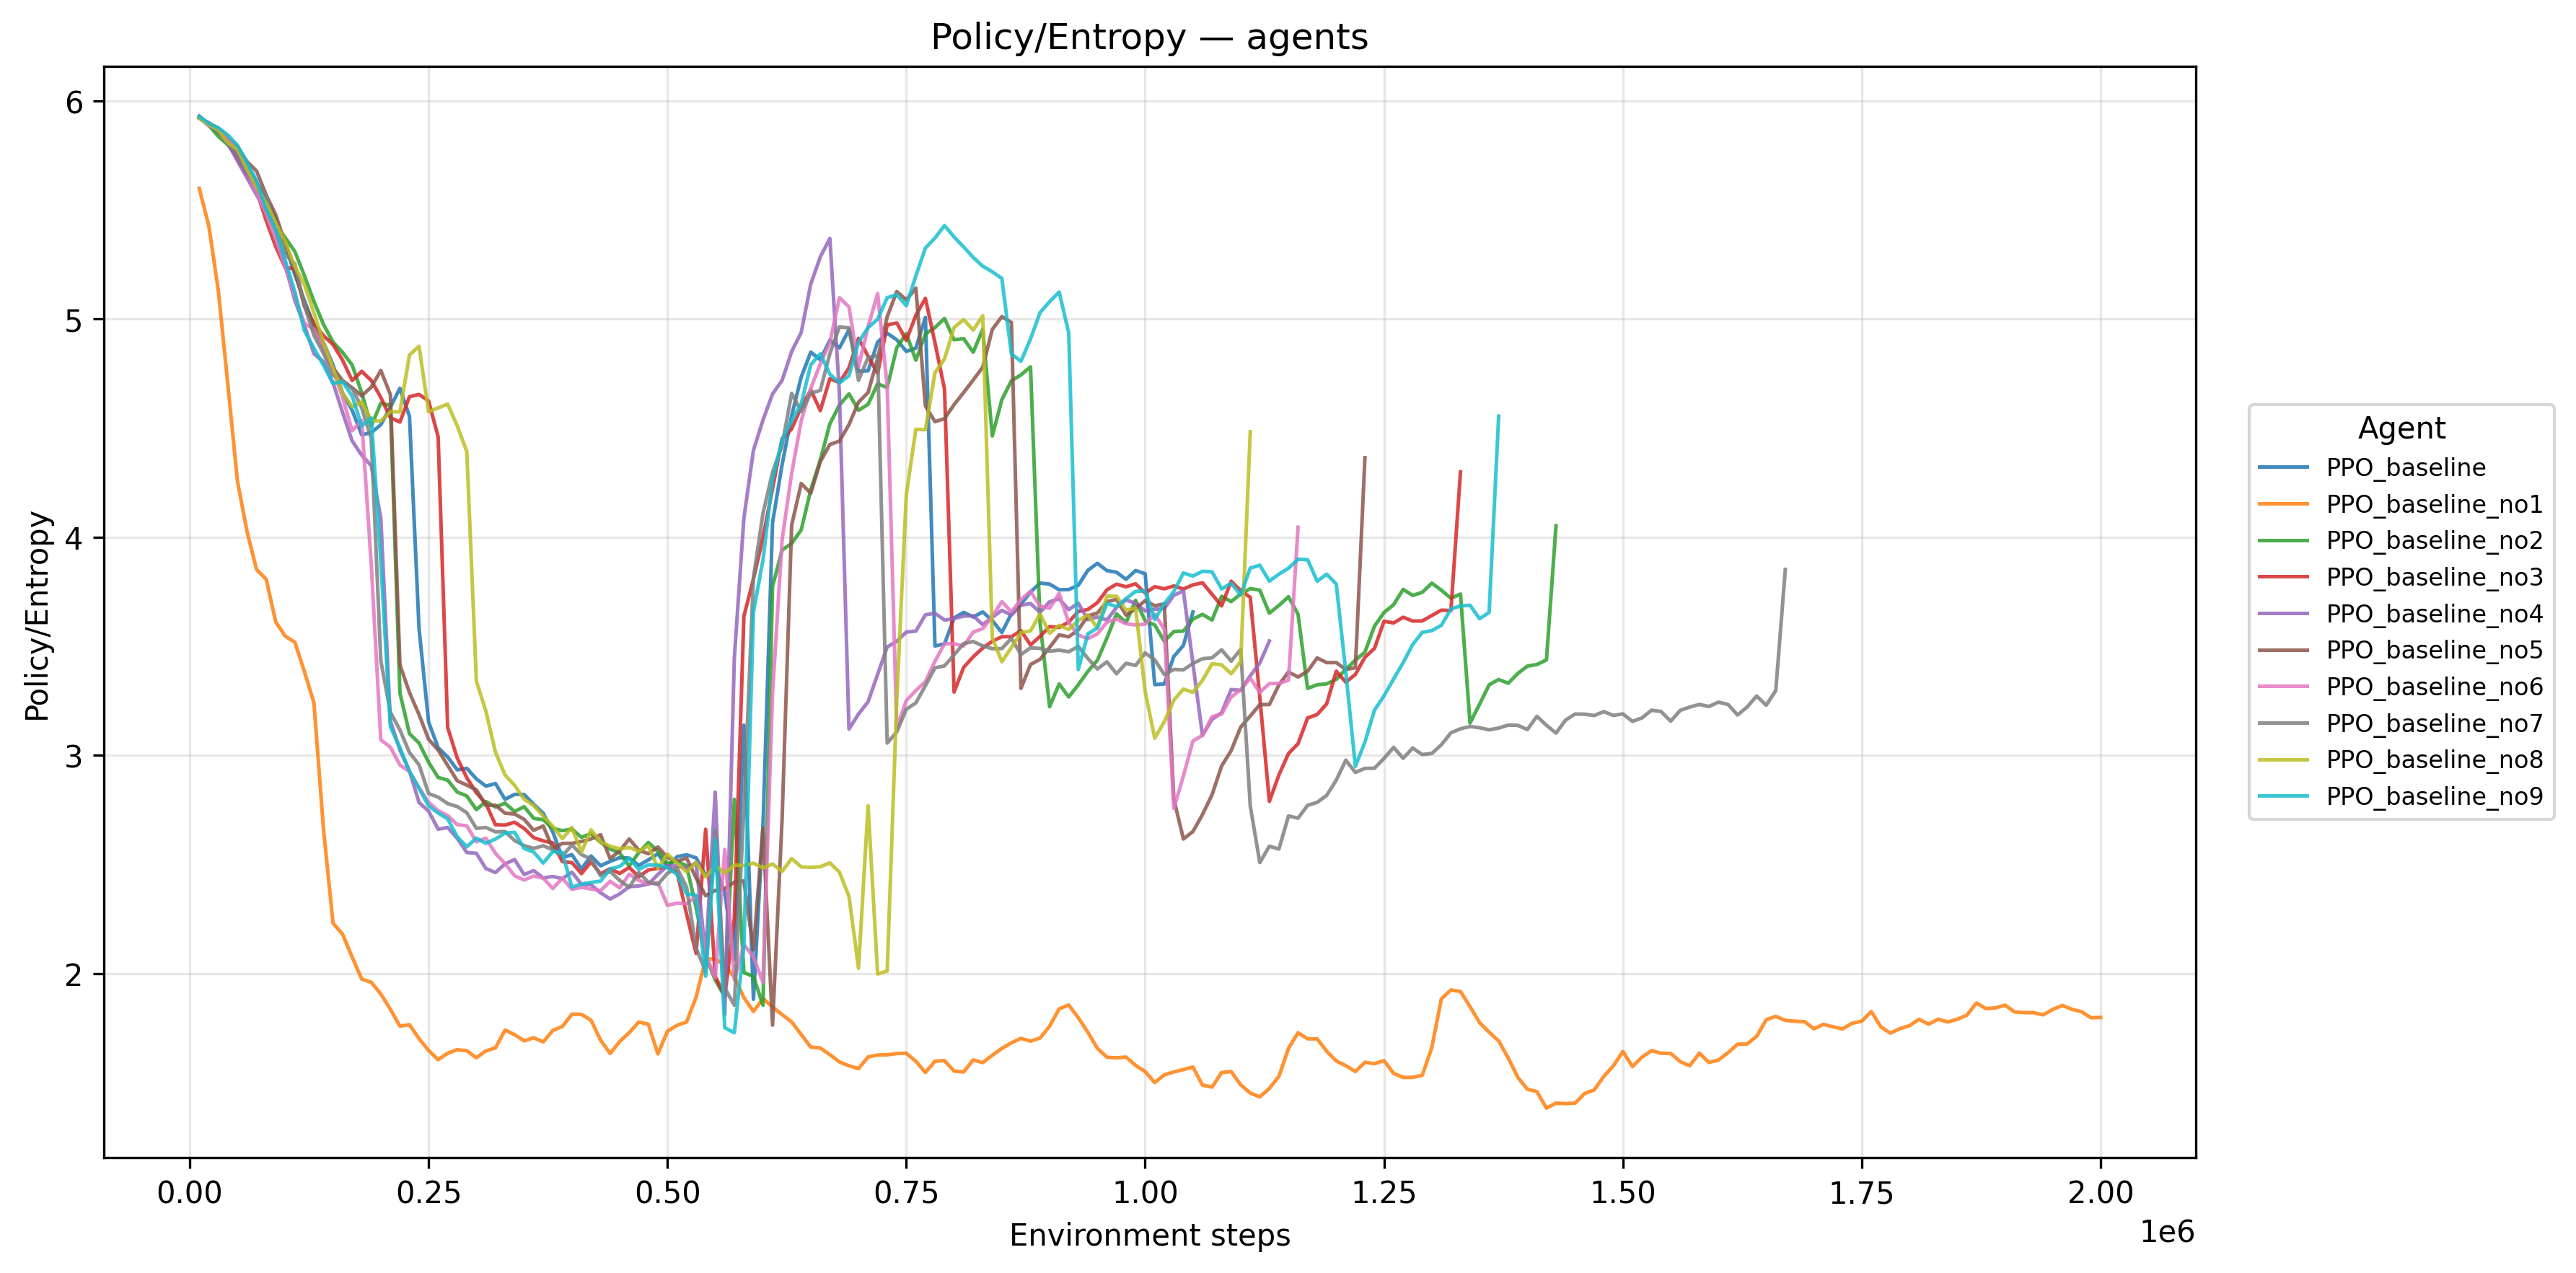
\includegraphics[width=1.0\textwidth]{images/baseline_results/Policy_Entropy_agents.png}
	%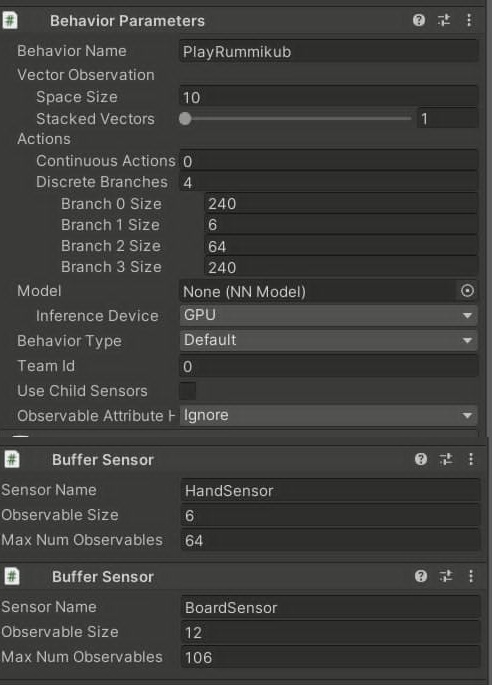
\includegraphics[width=0.7\textwidth]{images/BF_image.jpg}
	\caption{
		Entropy chart of individual 10 baseline agents
	}
	\label{fig:ppo_baseline_entropy}
\end{figure}

\begin{figure}[H]
	\centering
	
	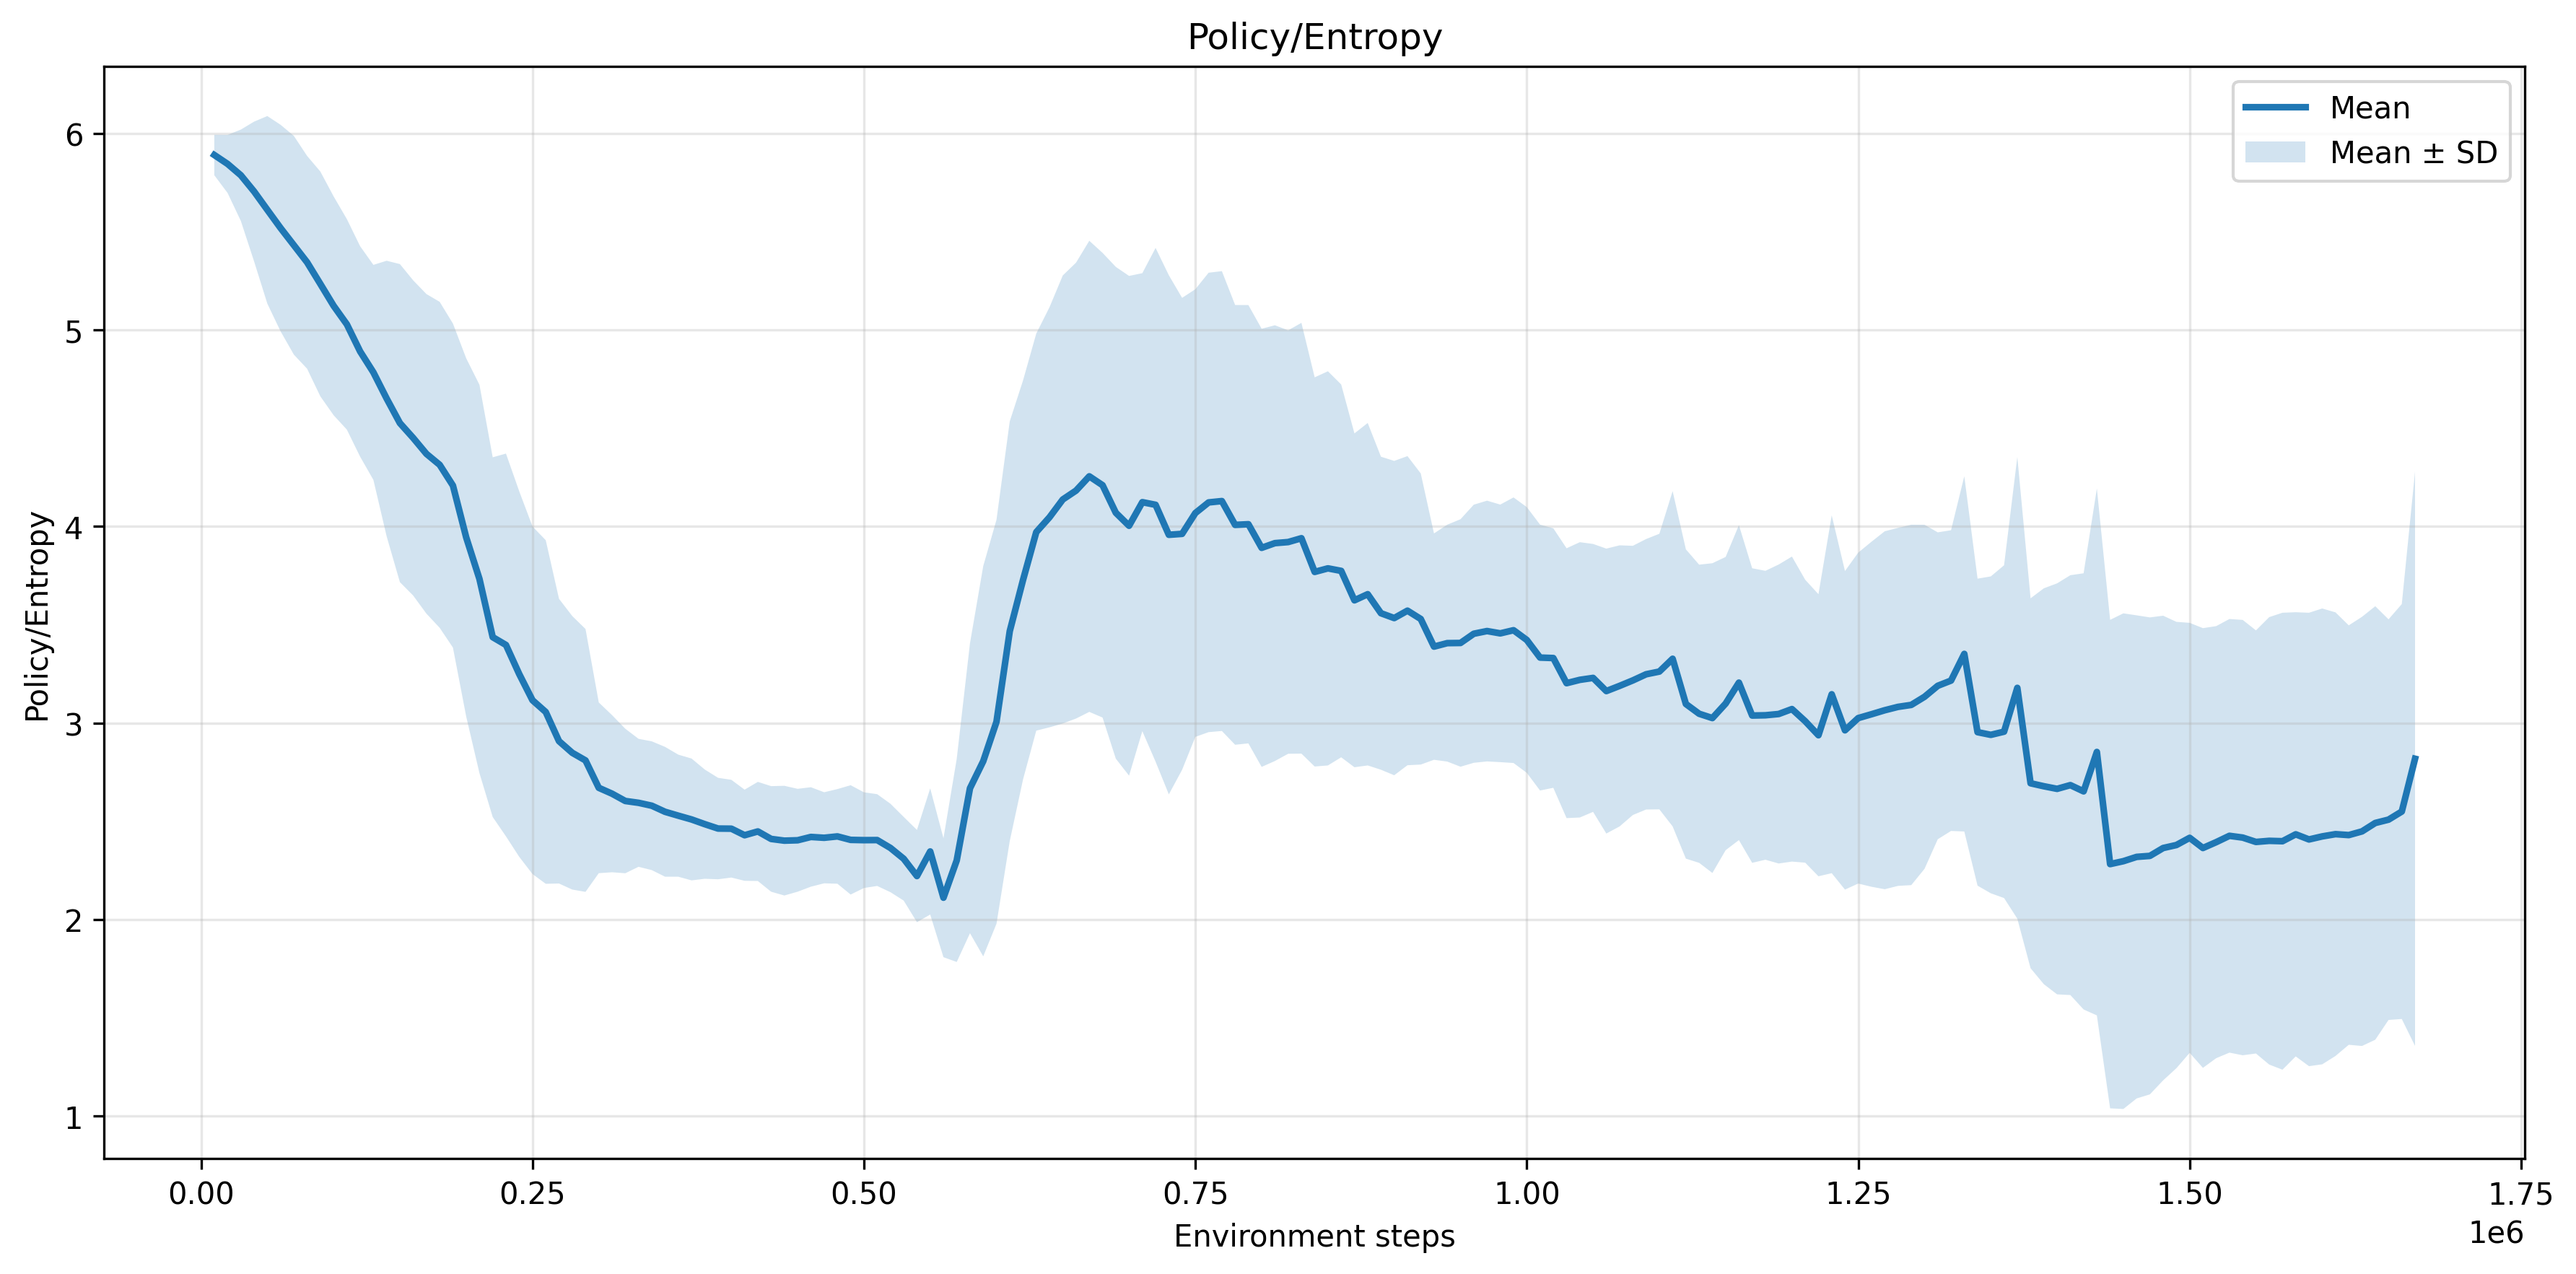
\includegraphics[width=1.0\textwidth]{images/baseline_results/Policy_Entropy_mean_sd.png}
	%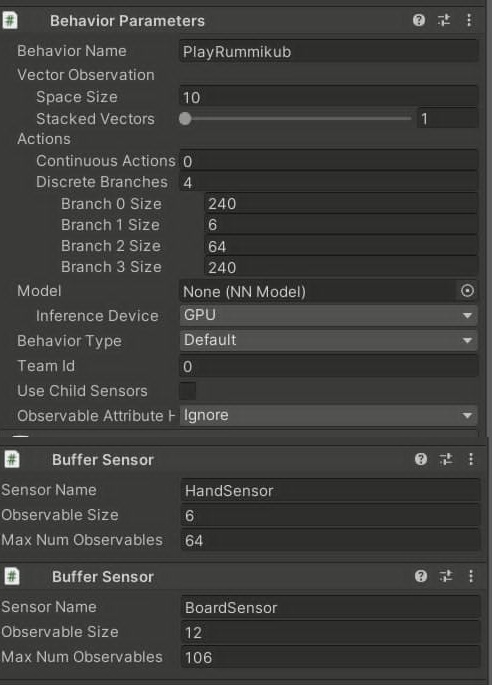
\includegraphics[width=0.7\textwidth]{images/BF_image.jpg}
	\caption{
		Entropy mean and SD chart of individual 10 baseline agents
	}
	\label{fig:ppo_baseline_entropy_mean_SD}
\end{figure}

The figure \ref{fig:ppo_baseline_entropy_mean_SD} summarizes the changes in policy entropy for the PPO Baseline agents. The initial decrease from around 5.9 to 2.3 shows that the policies changed gradually from highly exploratory behavior to more consistent action selection as the agents acquired the initial curriculum skills. The subsequent sharp increase at around 600,000 environment steps is suggestive of renewed exploration, prompted by the introduction of substantially more complex tasks. After this point, the mean entropy decreased gradually again, indicating the agents' policies progressively adapting and stabilizing.

The standard deviation band is relatively narrow during the period of lowest entropy, showing that the initial policies were developed similarly. It widens after the increase in task difficulty, indicating greater differences in exploration and adaptation between agents progressing through the curriculum at different rates. In the final part of the graph, the statistics are additionally influenced by the decreasing number of active training runs, since agents that have reached the target no longer produce further entropy observations.

\begin{table}[H]
	\centering
	\caption{
		First recorded training steps at which individual baseline agents completed the level.
	}
	\label{tab:baseline_level_intervals}
	
	\resizebox{\textwidth}{!}{%
		\begin{tabular}{
				c
				c c c c c c
				c c c c c c
			}
			\toprule
			
			\textbf{Run}
			& \textbf{L0}
			& \textbf{L1}
			& \textbf{L2}
			& \textbf{L3}
			& \textbf{L4}
			& \textbf{L5}
			& \textbf{L6}
			& \textbf{L7}
			& \textbf{L8}
			& \textbf{L9}
			& \textbf{L10}
			& \textbf{L11}
			\\
			
			\midrule
			
			0  & 240  & 560  & 580  & 580  & 590  &  590 & 590  & 600  & 600  &  780  & 1 010  & 1 050 \\
			1  & 140  & --   & --   & --   & --   & --   & --   & --   & --   & --    & --      & --\\
			2  & 220  & 530  & 570  & 570  & 580  & 580  & 580  & 600  & 610  & 880  & 1 320  & 1 430 \\
			3  & 260  & 520  & 540  & 540  & 550  & 550  & 550  & 570  & 580  & 790  & 1 120  & 1 330 \\
			4  & 200  & 540  & 550  & 550  & 560  & 560  & 560  & 570  & 570  & 680  & 1 050  & 1 130 \\
			5  & 210  & 580  & 600  & 600  & 610  & 610  & 610  & 620  & 620  & 860  & 1 030  & 1 230 \\
			6  & 190  & 540  & 560  & 560  & 570  & 570  & 570  & 600  & 610  & 730  & 1 020  & 1 160 \\
			7  & 200  & 520  & 550  & 550  & 560  & 560  & 560  & 580  & 580  & 720  & 1 110  & 1 670 \\
			8  & 300  & 690  & 710  & 710  & 720  & 720  & 720  & 730  & 740  & 840  & 1 000  & 1 110 \\
			9 & 200  & 530  & 550  & 550  & 560  & 560  & 560  & 580  & 590  & 910  & 1 210  & 1 360 \\
			
			\midrule
			
			\textbf{Mean}
			& 216 & 556.7 & 578.9 & 578.9 & 588.9 & 588.9
			& 588.9 & 605.6 & 611.1 & 798.9 & 1096.7 & 1274.4 \\
			
			\textbf{SD}
			& 41.03 & 50.5 & 49.5 & 49.5 & 49.5 & 49.5
			& 49.5 & 46.7 & 48.1 & 74.4 & 101.5 & 183.9\\
			
			\bottomrule
		\end{tabular}%
	}
	
%	\begin{minipage}{0.95\textwidth}
%		\footnotesize
%		Values are reported in thousands of environment steps. TensorBoard summaries were recorded every 10\,000 environment steps. Therefore, each value corresponds to the first recorded training step at which the given curriculum level was observed rather than the exact promotion step. A dash (--) indicates that the corresponding level was not reached during training. Mean and standard deviation were calculated only for agents that reached the corresponding curriculum level.
%	\end{minipage}
\end{table}
Values are reported in thousands of environment steps. TensorBoard summaries were recorded every 10\,000 environment steps. Therefore, each value corresponds to the first recorded training step at which the given curriculum level was observed rather than the exact promotion step. A dash (--) indicates that the corresponding level was not reached during training. Mean and standard deviation were calculated only for agents that reached the corresponding curriculum level.

The \textit{PPO\_baseline\_no1} agent exhibited a distinctly different entropy pattern. Its entropy decreased rapidly from around 5.6 to below 2.0 within the first 250,000 steps, then remaining between around 1.4 and 1.9 for most of the training process. Taken together with its curriculum-level progression, this shows that the agent maintained a considerably less exploratory policy while remaining at level 1. This may indicate premature convergence to an insufficient action-selection strategy to satisfy the promotion criterion.

The remaining agents maintained higher entropy values and continued to progress through the curriculum. Temporary increases near the end of several training runs appear to coincide with transitions to more difficult levels. Overall, the results suggest that successful agents repeatedly increased their level of exploration in response to changes in the curriculum, subsequently reducing or stabilizing it as they adapted to new tasks. In contrast, the unsuccessful \textit{PPO\_baseline\_no1} agent maintained relatively low entropy and did not progress beyond level 1.

The table \ref{tab:baseline_level_intervals} presents the first recorded training steps at which the individual PPO baseline agents reached successive curriculum levels. Nine out of ten agents reached level 12. The only unsuccessful run was agent 1, which reached level 1 after approximately 140,000 environment steps but did not progress to any subsequent level within the training budget.

On average, the agents reached level 1 after taking 216,000 steps in the environment. Reaching level 2 required substantially more training, with an average of around 556,700 steps. The difference of around 340,700 steps between the mean values for levels 1 and 2 suggests that level 1 was the first significant hurdle in the curriculum. However, the relatively low standard deviation of around 50,500 steps for reaching level 2 suggests that the successful agents experienced a similar degree of difficulty at this stage.

After reaching level 2, the successful agents progressed rapidly through the subsequent intermediate levels. The mean number of steps recorded increased from around 556,700 at level 2 to just 611,100 at level 9. In several cases, the same number of steps was recorded for multiple consecutive levels. This does not necessarily mean that the levels were completed at exactly the same training step. As TensorBoard summaries were recorded every 10,000 environment steps, multiple curriculum transitions could occur within a single recording interval.

An increase in training requirements was observed for later stages of the curriculum. On average, level 10 was reached after approximately 798,900 steps, while level 11 required an average of approximately 1,096,700 steps. This difference of around 297,800 steps indicates that Level 10 was one of the most demanding stages in the curriculum. Level 12 was reached after an average of around 1,274,400 steps in the environment.

Variability between successful agents increased at the later stages of the curriculum. The standard deviation rose from approximately 48,100 steps for level 9 to 74,400 for level 10, 101,500 for level 11, and 183,900 for level 12. Agent 0 reached level 12 first, after approximately 1,050,000 steps, whereas agent 7 required approximately 1,670,000 steps. The difference of 620,000 steps between these runs demonstrates considerable variation in learning speed despite the use of the same training configuration.

Overall, the results suggest that levels 1, 9, 10 and 11 required the most training, while levels 2–8 were completed relatively quickly by the successful agents. The increasing standard deviation at later stages further suggests that agents' abilities to adapt differed more strongly as the curriculum tasks became more complex.
\begin{table}[H]
	\centering
	\caption{
		Training outcome of individual PPO baseline agents.
	}
	\label{tab:baseline_training_time}
	
	\begin{tabular}{c c c c}
		\toprule
		
		\textbf{Agent}
		&
		\textbf{Training stopped at step}
		&
		\textbf{Target reached}
		&
		\textbf{Training time [h]}
		\\
		
		\midrule
		
		0  & 1 050 & Yes & 3.83 \\
		1  & 2 000 & No & 9.16 \\
		2  & 1 430 & Yes & 5.41 \\
		3  & 1 330 & Yes & 4.96 \\
		4  & 1 130 & Yes & 4.12 \\
		5  & 1 230 & Yes & 4.48 \\
		6  & 1 160 & Yes & 3.98 \\
		7  & 1 670 & Yes & 5.95 \\
		8  & 1 110 & Yes & 4.03 \\
		9  & 1 360 & Yes & 5.27 \\
		
		\midrule
		
		\textbf{Mean}
		&
		1347
		&
		90\%
		&
		5.12 \\
		
		\textbf{SD}
		&
		278.96
		&
		
		&
		1.5 \\
		
		\bottomrule
	\end{tabular}
	
	%\begin{minipage}{0.95\textwidth}
		%\footnotesize
		%Training stopped indicates the first recorded training step at which curriculum level 12 was reached or the predefined training limit of 2 million environment steps if the target was not achieved. Target reached denotes whether the agent successfully reached the predefined target curriculum level. Training time is reported as the total active training time in hours.
	%\end{minipage}
	
\end{table}

%The table \ref{tab:baseline_training_time} 
Training stopped indicates the first recorded training step at which curriculum level 12 was reached or the predefined training limit of 2 million environment steps if the target was not achieved. Target reached denotes whether the agent successfully reached the predefined target curriculum level. Training time is reported as the total active training time in hours.

The table \ref{tab:baseline_training_time} summarizes the training outcomes of the ten agents using the PPO baseline configuration. Nine of the agents reached the predefined target level, giving a success rate of 90\%. Agent 1 was the only unsuccessful run. Its training continued until the predefined limit of two million environment steps, lasting 9.16 hours, but did not reach the target.

Of the successful runs, Agent 0 took the shortest time to reach the target, achieving this after approximately 1,050,000 environment steps and 3.83 hours of training. Agent 7 took the most steps of all the successful agents to reach the target, doing so after approximately 1,670,000 steps and 5.95 hours. The difference between the fastest and slowest successful runs was therefore approximately 620,000 environment steps and 2.12 hours. 
While the recorded training time was generally associated with the number of environment steps required to reach the target, the relationship was not strictly proportional. For example, Agent 4 reached the target after around 1,130,000 steps in 4.12 hours, whereas Agent 8 reached it earlier, after around 1,110,000 steps, but still required 4.03 hours. By contrast, Agent 6 completed around 1,160,000 steps in just 3.98 hours. Thus, although agent 6 required more environment steps than agents 4 and 8, it completed its training in less wall-clock time.

This difference suggests that training duration is also affected by variations in computational throughput. 
%Factors such as temporary CPU and GPU load, the computational cost of individual episodes, parallel environment execution, checkpoint operations and other processes running on the training device could influence the number of environment steps processed per hour. Consequently, the number of steps should be treated as the primary measure of learning speed, as it represents the amount of experience collected by the agent.
Wall-clock training time, on the other hand, describes the practical computational cost of conducting a training run under the available hardware conditions.

When all ten runs are considered, training stopped after an average of approximately 1,347,000 environment steps, with a standard deviation of approximately 278,960 steps. The average training time was 5.12 hours, with a standard deviation of 1.50 hours. However, these aggregate values include the unsuccessful agent, whose training continued until the maximum step limit. Consequently, they describe the overall computational cost of the experiment rather than the average time required to reach the target.

\subsubsection{Evaluation results}
The table \ref{tab:baseline_evaluation_results} presents the evaluation results of the ten PPO baseline agents. Each agent was evaluated over 1,000 independent episodes on curriculum level 11, resulting in a total of 10,000 evaluation episodes.
\begin{table}[H]
	\centering
	\caption{Evaluation results of PPO baseline agents over 1000 episodes on curriculum level 11.}
	\label{tab:baseline_evaluation_results}
	\begin{tabular}{c r r r r}
		\toprule
		\textbf{Agent} &
		\textbf{Episodes} &
		\textbf{Wins} &
		\textbf{Losses} &
		\textbf{Win rate [\%]} \\
		\midrule
		0 & 1000 & 721 & 279 & 72.10 \\
		1 & 1000 & 354 & 646 & 35.40 \\
		2 & 1000 & 703 & 297 & 70.30 \\
		3 & 1000 & 631 & 369 & 63.10 \\
		4 & 1000 & 714 & 286 & 71.40 \\
		5 & 1000 & 670 & 330 & 67.00 \\
		6 & 1000 & 685 & 315 & 68.50 \\
		7 & 1000 & 675 & 325 & 67.50 \\
		8 & 1000 & 651 & 349 & 65.10 \\
		9 & 1000 & 705 & 295 & 70.50 \\
		\midrule
		\textbf{Total} &
		\textbf{10\,000} &
		\textbf{6509} &
		\textbf{3491} &
		\textbf{} \\
		\textbf{Mean} &
		 &
		 &
		 &
		65.09 \\
		\textbf{SD} &
		 &
		 &
		 &
		10.26 \\
		\bottomrule
	\end{tabular}
\end{table}
Collectively, the agents achieved 6,509 wins and 3,491 losses, giving them an average win rate of 65.09\%. The standard deviation of the individual agents' win rates was 10.26 percentage points, indicating variation in evaluation performance between the trained policies.

Agent 0 achieved the highest win rate of 72.10\%, followed by agent 4 with 71.40\%, agent 9 with 70.50\%, and agent 2 with 70.30\%. Among the agents that reached the predefined target during training, the lowest evaluation result was obtained by agent 3, with a win rate of 63.10\%. Therefore, the win rates of the successful training runs ranged from 63.10\% to 72.10\%. This relatively limited range indicates that agents that successfully completed the target training stage generally acquired policies of comparable effectiveness, despite the previously observed differences in learning speed.

Agent 1 produced a distinctly lower win rate of 35.40\%. This was also the only agent that did not reach the predefined target level during training, as it remained at curriculum level 1 until the training limit was reached. Its considerably weaker evaluation result is therefore consistent with its incomplete curriculum progression. Nevertheless, the agent was still able to win some evaluation episodes, suggesting that the strategies learned during the initial curriculum stages provided limited transferable capabilities or that some level 11 instances could be solved without a fully developed policy.

Overall, the evaluation results indicate that reaching the predefined curriculum target was associated with substantially better performance on level 11. However, reaching the target did not result in perfect task execution, as even the best-performing agent lost approximately 28\% of its evaluation episodes. The results therefore demonstrate that the agents acquired useful and relatively consistent strategies, while leaving room for further improvement in policy reliability.
\subsection{GAIL as auxiliary method}
This section presents the results of the model during the training process, as well as the final evaluation results of the GAIL model.
\subsubsection{Learning results}
Figure \ref{fig:gail_CumulativeReward} shows a graph of \textbf{Cumulative Rewards} obtained during the training of ten independent agents using the \textbf{GAIL} auxiliary method. In the initial training interval, between 0 and 200,000 steps, there is a rapid increase in the environment’s reward, with each agent exhibiting a very similar rate of increase. Once the agents achieved scores close to 0.5, there was a sharp drop in the reward, which may indicate that the agent advanced to the next level, where it encountered difficulties. This pattern repeats throughout the entire training process, the environment reward rises and then suddenly drops. This may indicate that the agent is successfully progressing to subsequent levels, where it must readjust its policy to accommodate the increasing difficulty of the tasks.

After around 200,000 steps, the learning trajectories of the agents begin to diverge. Declines and returns to positive rewards occur at different times, some agents experience steeper declines in environmental rewards and complete training after varying numbers of steps.

Among all runs, agent \textit{PPO\_GAIL\_no9} draws particular attention, as it experienced a sharp drop in the environmental reward around the 900,000th step. A similar phenomenon was observed in the case of agent \textit{PPO\_GAIL} around the 1.1 millionth step. These drops may indicate short-term policy instability or difficulties in adapting the policy to changing environmental conditions. In both cases, however, the reward was gradually restored and returned to positive values. This suggests that the observed deterioration was temporary and did not lead to a permanent breakdown of the learning process.


\begin{figure}[H]
	\centering
	
	%\figureplaceholder{
	%	Placeholder: GAIL cumulative reward
	%}
	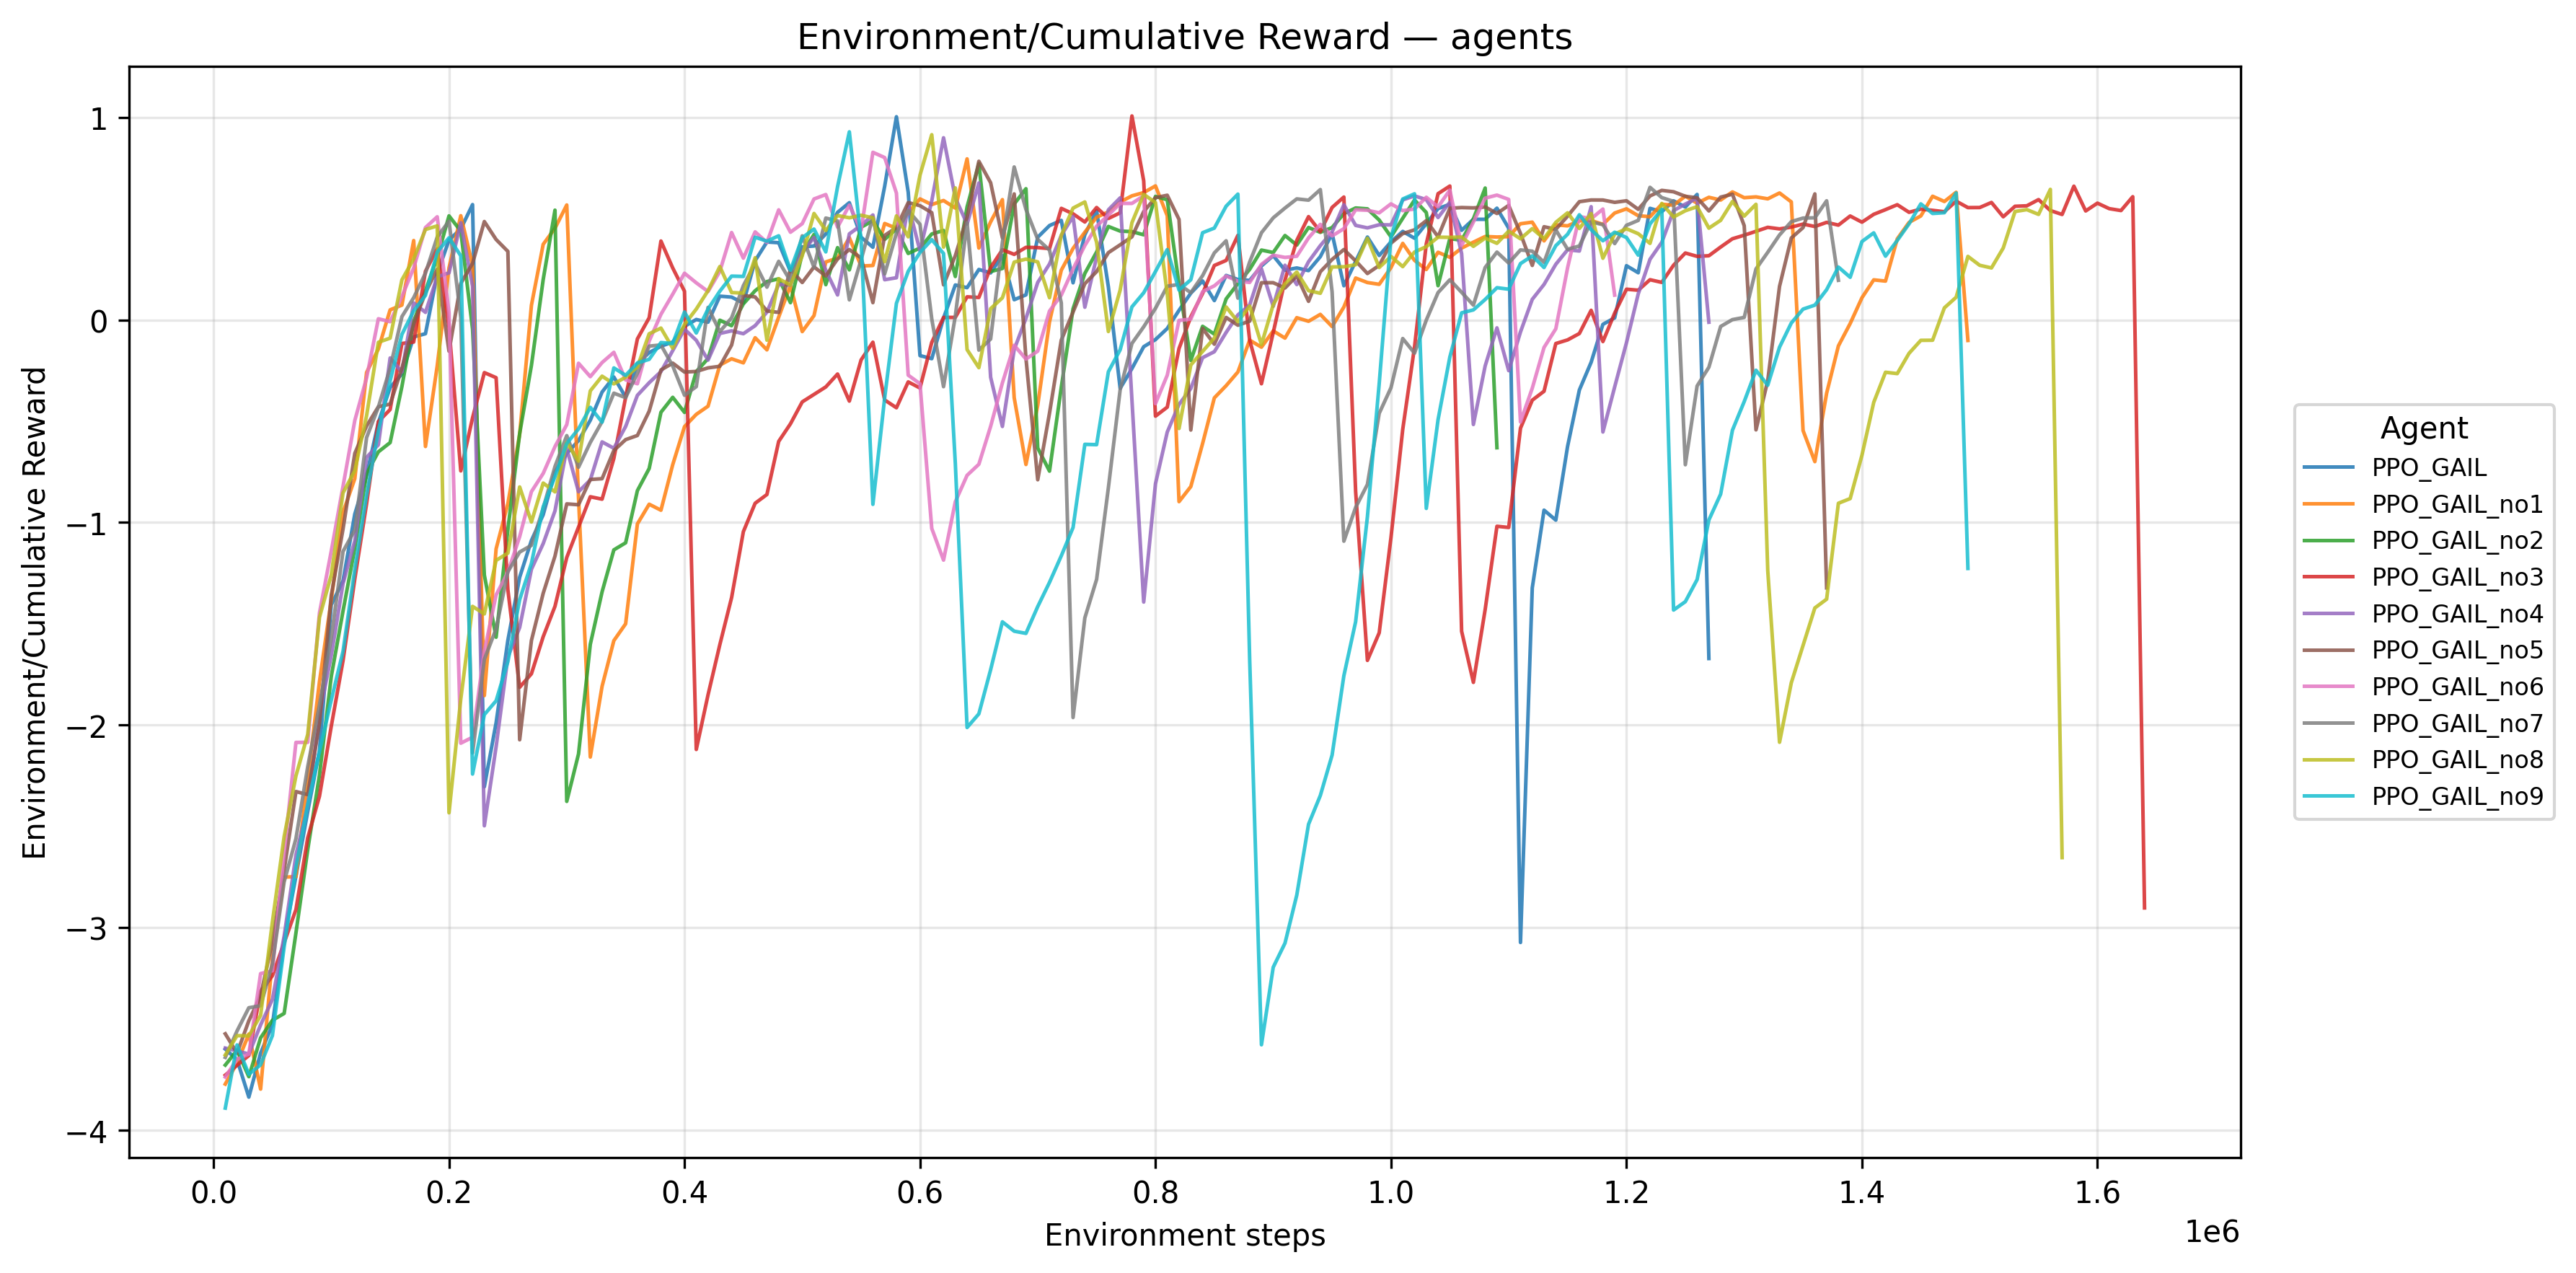
\includegraphics[width=1.0\textwidth]{images/gail_results/Environment_Cumulative_Reward_agents.png}
	\caption{
		Cumulative reward graph of 10 GAIL agents
	}
	\label{fig:gail_CumulativeReward}
\end{figure}


Nevertheless, given that every agent completed training before reaching 2 million steps, it can be concluded that each agent ultimately reached the expected level.

Figure \ref{fig:gail_lessonNumber} displays the stage and time at which each of the ten GAIL agents was at, as well as when they advanced to the next level. The first promotions occurred after just 200,000 steps, with the agent \textit{PPO\_GAIL\_no3} being the last to be promoted, advancing to level one after 400,000 steps. Level zero marked the beginning of the learning process, so it is understandable that initially grasping the rules of the game might take more time. 

Subsequent level-ups occurred within the range of 500,000 to 750,000. Once the conditions for promotion to a higher level were met, a sudden increase in levels could be observed. This suggests that levels 2 through 8 were similar enough that, after mastering levels 0 and 1, agents did not need to adjust their approach to meet the promotion criteria.

Figure \ref{fig:gail_CumulativeReward_mean_SD} summarizes the curriculum rewards obtained by the PPO+GAIL agents. The mean reward increased rapidly from approximately $-3.7$ to positive values within the first 200,000 environment steps, indicating that the agents generally acquired the initial curriculum skills. The subsequent sharp decrease and gradual recovery reflect adaptation to more difficult tasks. During the remaining training period, the mean reward fluctuated mainly around zero and positive values, showing repeated adaptation as the agents progressed through the curriculum.



\begin{figure}[H]
	\centering
	
	%\figureplaceholder{
		%	Placeholder: GAIL cumulative reward
		%}
	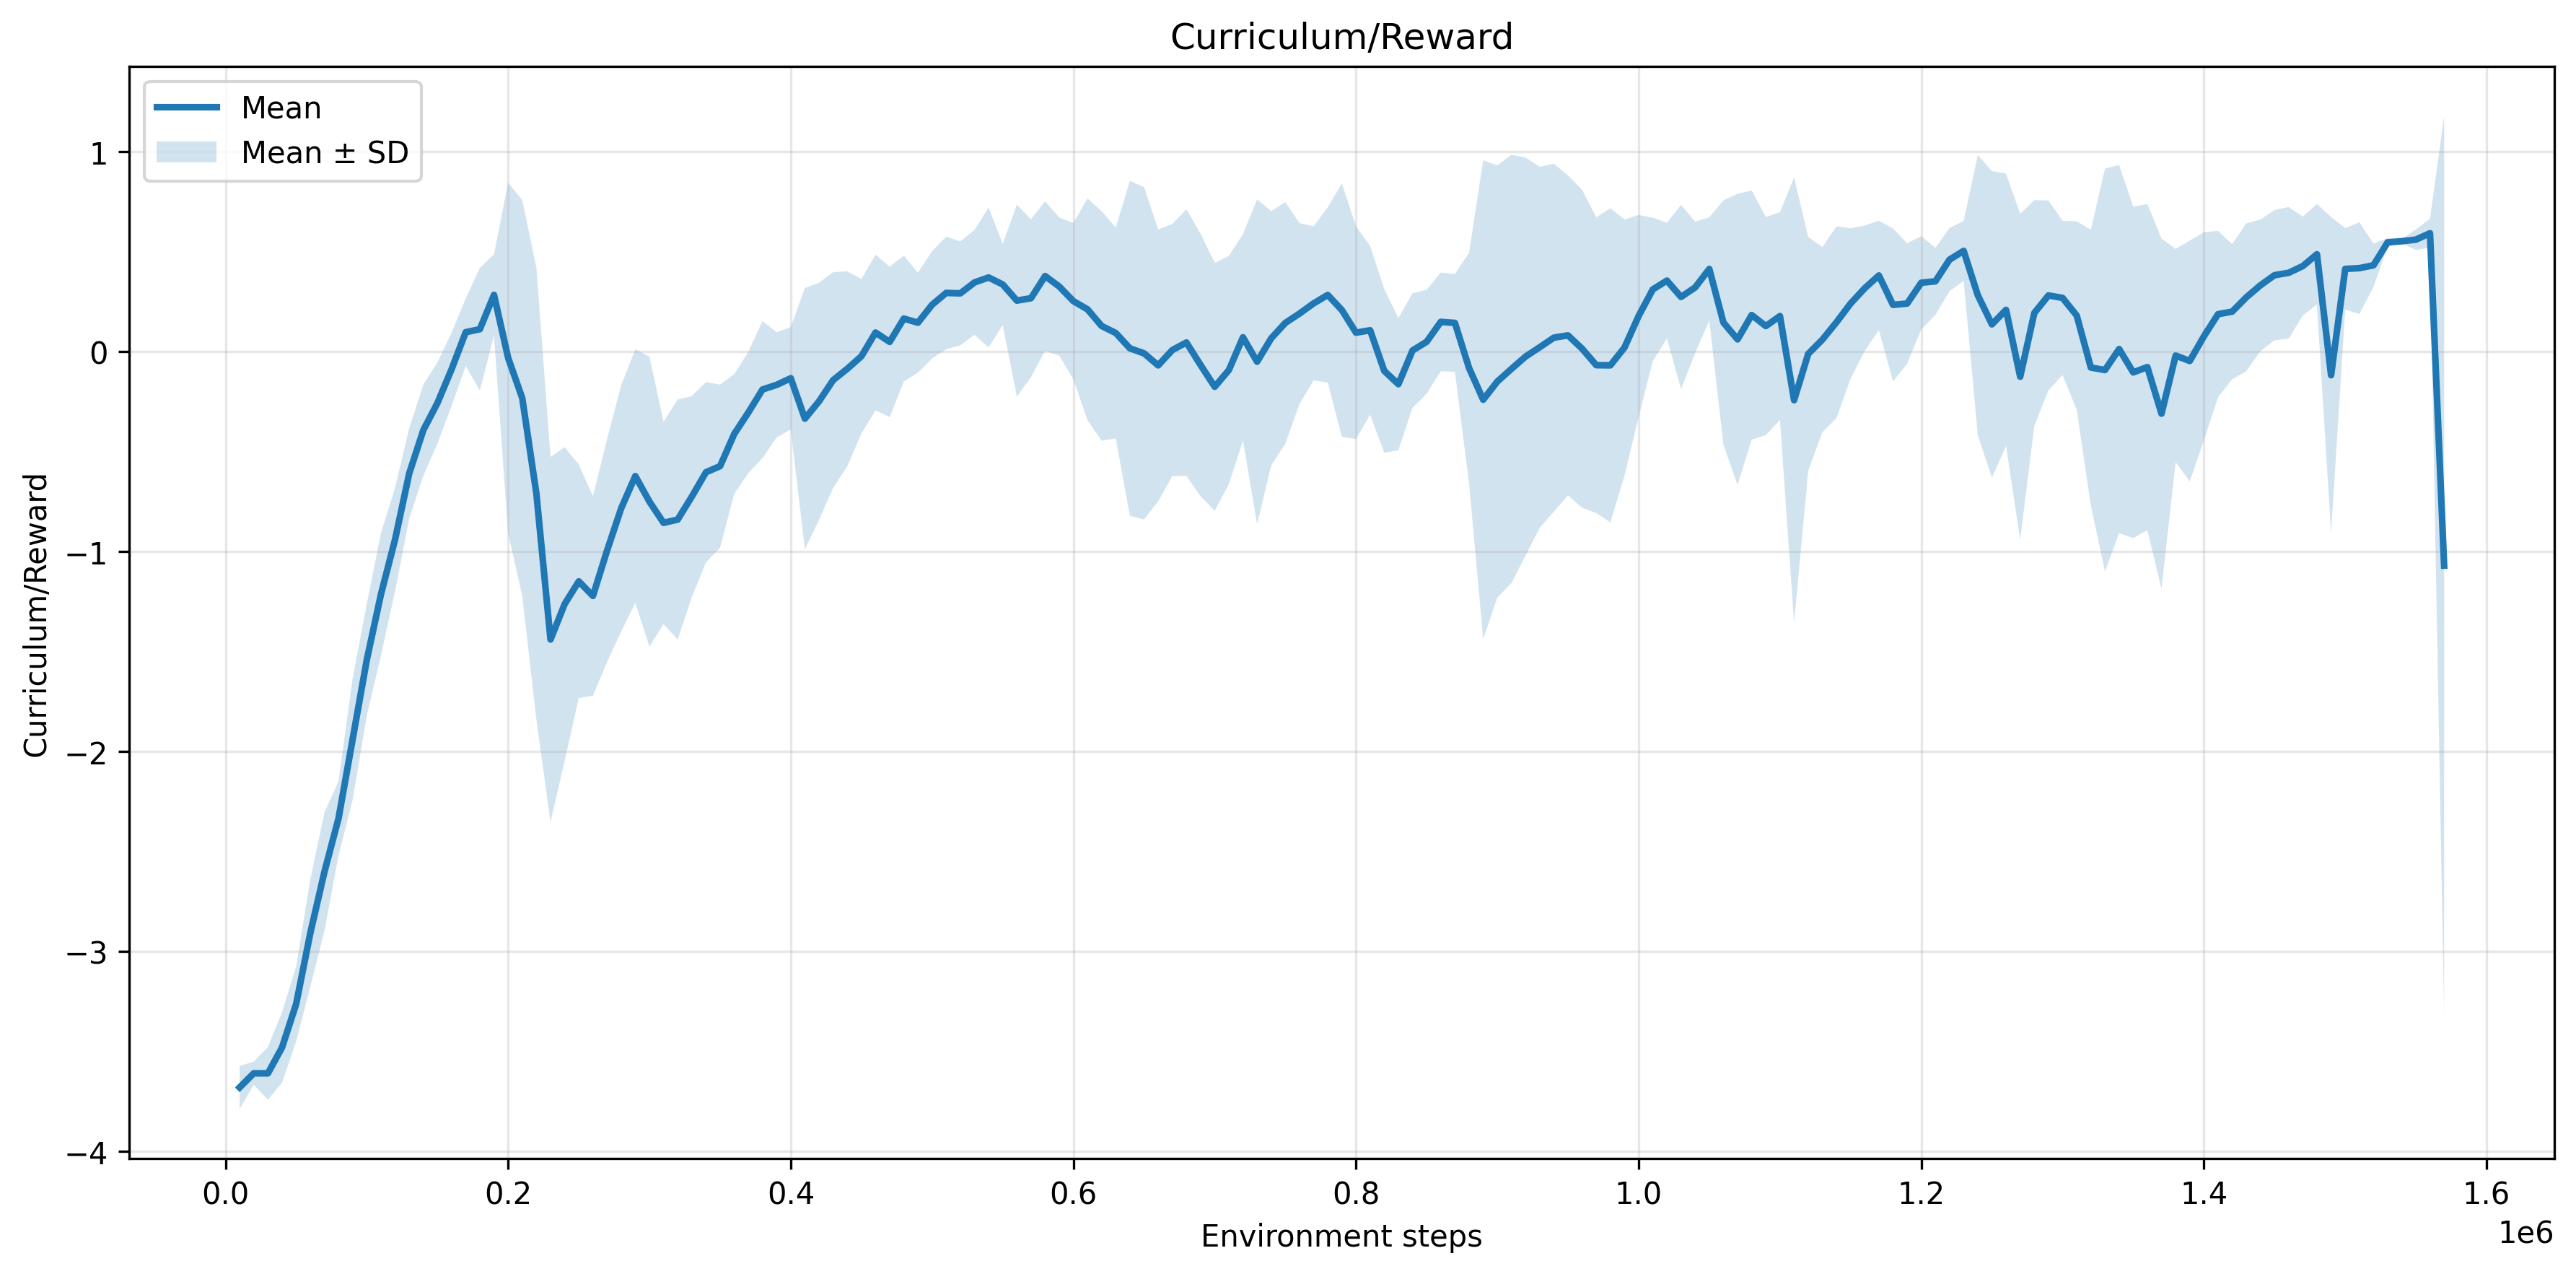
\includegraphics[width=1.0\textwidth]{images/gail_results/Curriculum_Reward_mean_sd.png}
	\caption{
		Cumulative reward graph of 10 GAIL agents
	}
	\label{fig:gail_CumulativeReward_mean_SD}
\end{figure}

The standard-deviation band becomes wider after the initial stage, indicating differences in the moments at which agents entered and adapted to more difficult tasks. Nevertheless, all PPO+GAIL agents ultimately reached the training target. The abrupt change at the end of the graph should not be interpreted as a deterioration of the entire group because, by that point, most agents had already completed training, and the calculated statistics were based only on the remaining active runs.

\begin{figure}[H]
	\centering
	
	%\figureplaceholder{
	%	Placeholder: GAIL curriculum progression
	%}
	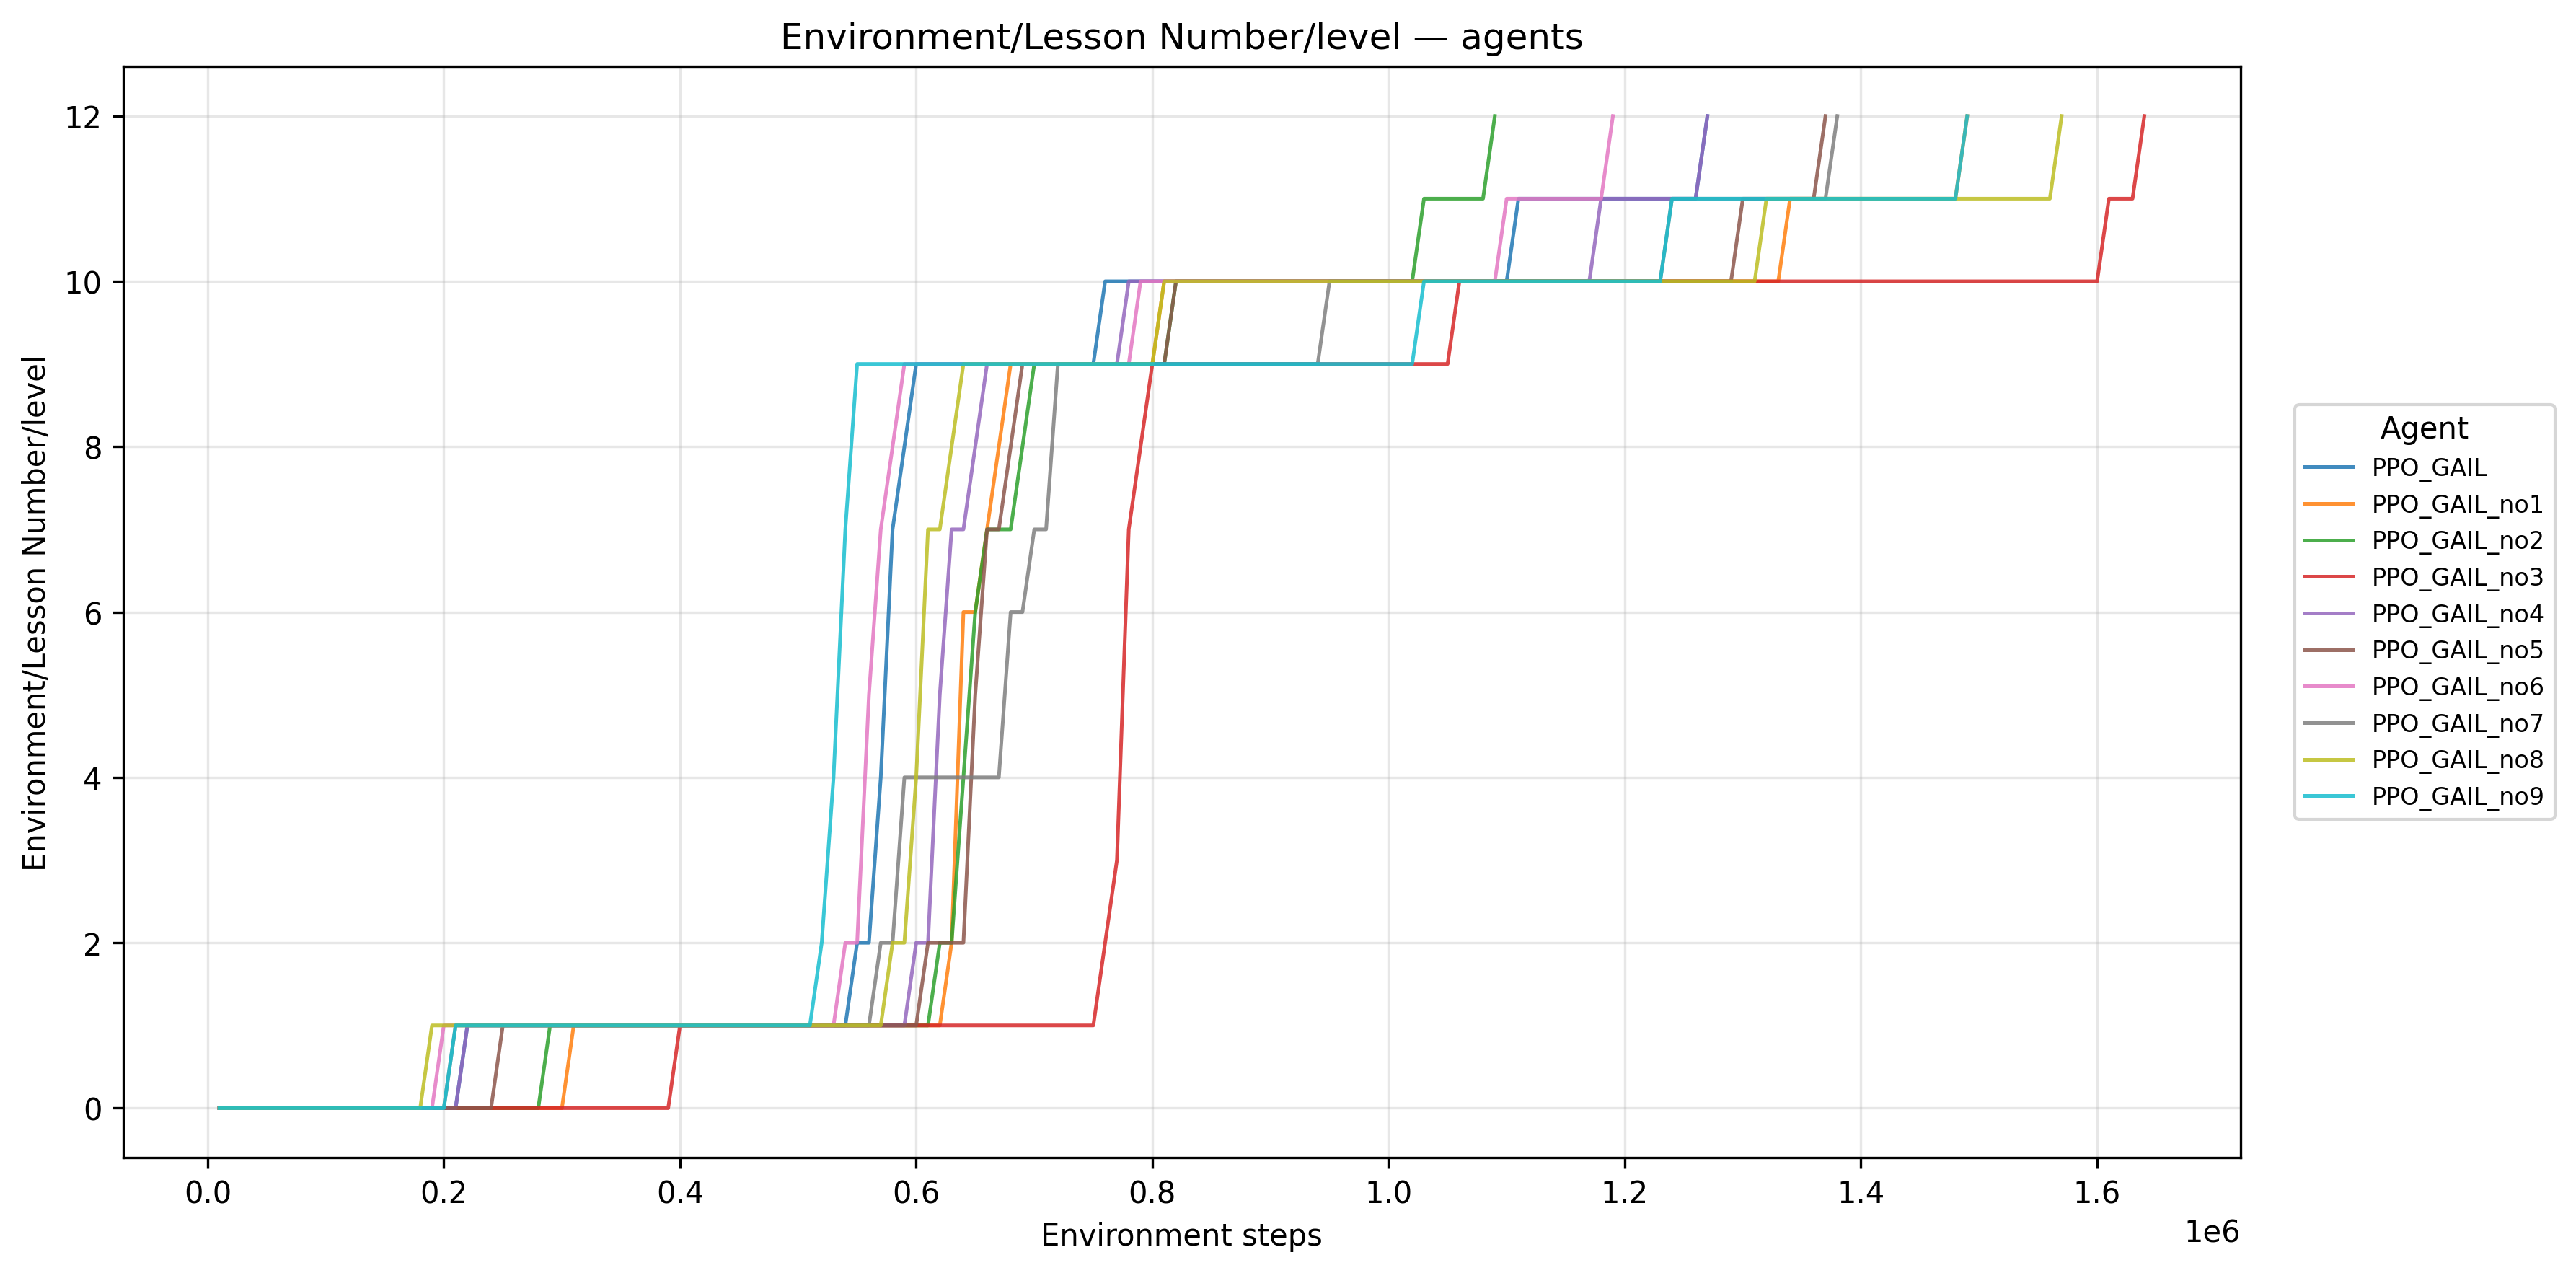
\includegraphics[width=1.0\textwidth]{images/gail_results/Environment_Lesson_Number_level_agents.png}
	\caption{
		lesson progress graph of 10 GAIL agents
	}
	\label{fig:gail_lessonNumber}
\end{figure}

Level 9 presented another challenge, requiring the agent to spend more time meeting the promotion requirements. The task begins with the agent placing a sequence on the board, while another completed sequence is already present on the map. This represents a significant change for the agent, as in previous levels there was only one sequence on the map. This explains why more time was spent on this task. Agents advanced at different times, some advanced between 770,000 and 800,000, while others needed more time and did not advance until they reached between 950,000 and 1,050,000.

Referring to the plot \ref{fig:gail_CumulativeReward} of \textbf{Cumulative Rewards}, it can be seen that the agent \textit{PPO\_GAIL\_no9} had already been at level 9 for some time by the 900,000th step and did not advance to level 10 until around the 1.03 millionth step. This may indicate that the significant decrease in the environmental reward during this period may have been caused by short-term policy instability. Ultimately, however, the reward was restored, and the agent eventually met the criteria for promotion to level 10, suggesting that there was no permanent breakdown in the agent’s policy.

However, the situation was different for agent \textit{PPO\_GAIL}, which experienced a similar sudden drop around 1.1 million steps \ref{fig:gail_CumulativeReward}. However, as shown in Figure \ref{fig:gail_lessonNumber}, this drop in performance was influenced by an advancement to a higher level, which is to be expected during the learning process.

As agents progress to Level 10, their differences become more apparent. While some agents progress to Level 11 quickly, others remain at Level 10 for a considerable amount of time. Spending a long time at Level 10 is consistent with the nature of the task. The agent must place two items in the presence of a complete sequence, requiring them to perform several correct, interdependent actions. This is more challenging than adding a single missing item at Level 9.

Level 11 also has characterized by varying completion times. While some agents complete it relatively quickly, while others spend more time on it. For example, agents \textit{PPO\_GAIL\_no2} and \textit{PPO\_GAIL\_no3} completed Level 11 relatively quickly. Conversely, agents \textit{PPO\_GAIL\_no9} and \textit{PPO\_GAIL\_no8} took longer to successfully learn Level 11. Agent \textit{PPO\_GAIL\_no2} completed the training the fastest, requiring approximately 1.1 million steps to complete Level 11. In contrast, agent \textit{PPO\_GAIL\_no3} took the longest, requiring 1.65 million steps. The difference between them is as much as 550,000 steps.

Agent \textit{PPO\_GAIL\_no3} is particularly noteworthy, as he was the last to reach each level compared to the other agents. Another interesting case is agent \textit{PPO\_GAIL\_no9}, who advanced the fastest from level 1 to level 9. He spent a long time at level 9 despite his rapid advancement during the earlier stages of learning.

Overall, the GAIL auxiliary method allowed all agents to reach the desired outcome. However, it did not eliminate significant variability in the learning rate or short-term declines in performance at an unchanged level of the curriculum.

\begin{figure}[H]
	\centering
	
	%\figureplaceholder{
		%	Placeholder: GAIL curriculum progression
		%}
	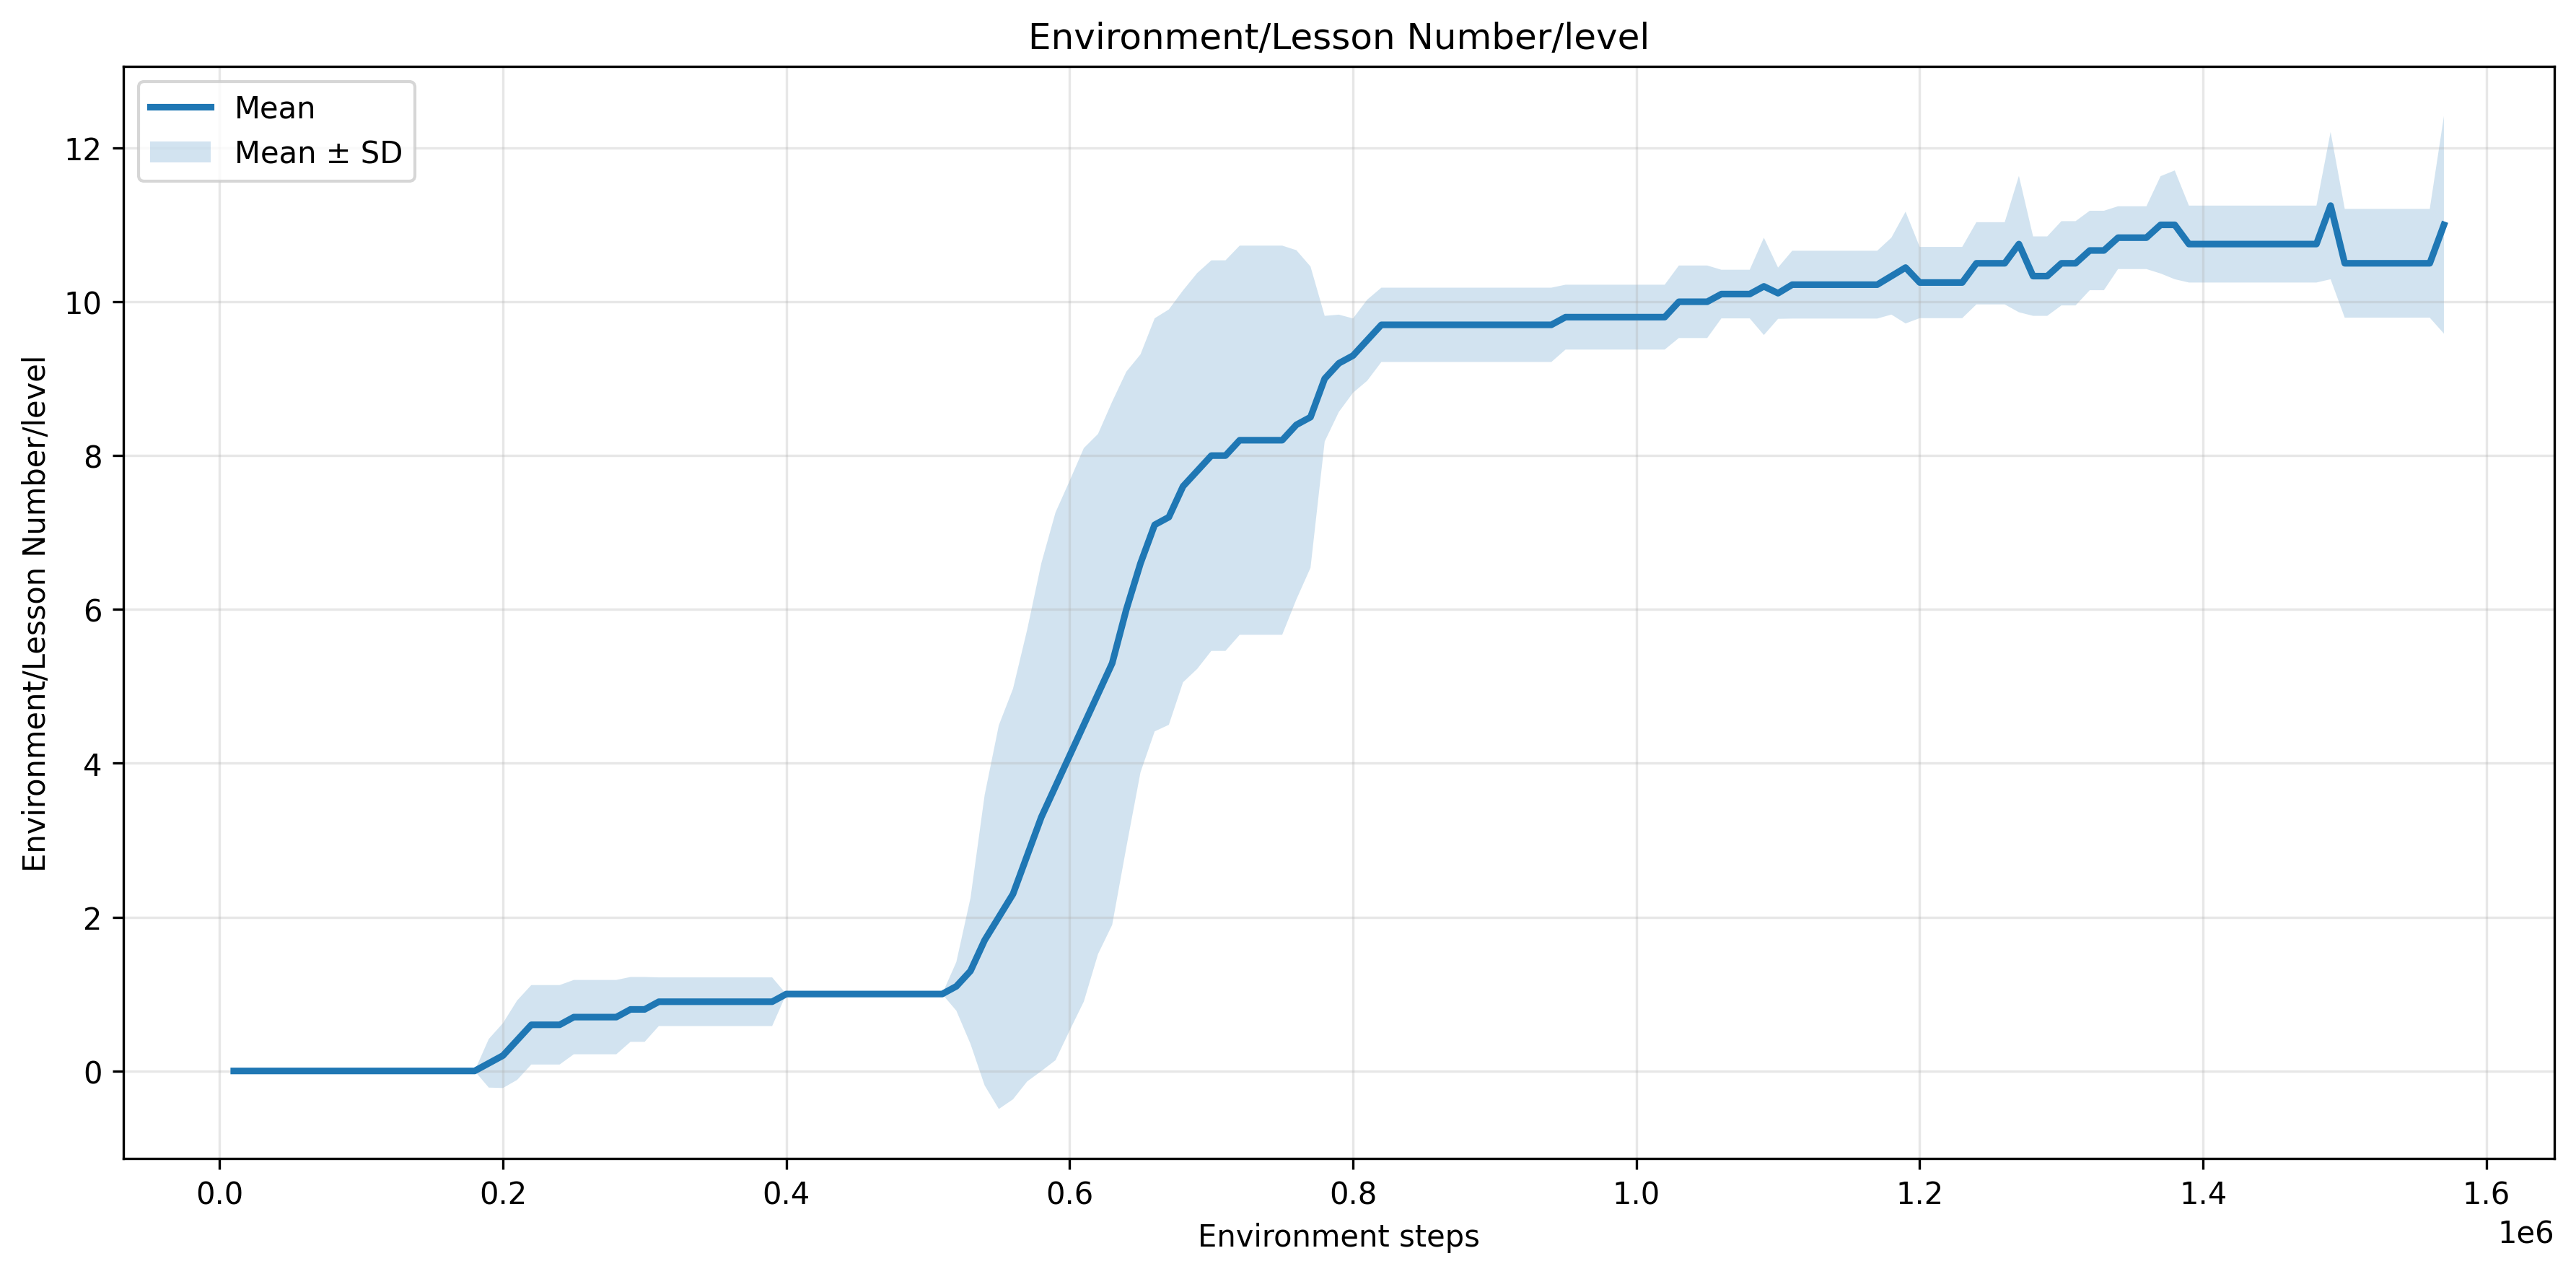
\includegraphics[width=1.0\textwidth]{images/gail_results/Environment_Lesson_Number_level_mean_sd.png}
	\caption{
		lesson progress mean and SD graph of 10 GAIL agents
	}
	\label{fig:gail_lessonNumber_mean_SD}
\end{figure}
Figure \ref{fig:gail_lessonNumber_mean_SD} summarizes the curriculum progression of the PPO+GAIL agents. The mean lesson number remained low during the initial training stage and then increased rapidly between approximately 500,000 and 800,000 environment steps. After reaching the later curriculum tasks, the progression became slower, indicating that these skills required substantially more experience than the earlier tasks.

The standard-deviation band is widest during the rapid progression through the intermediate lessons, showing that individual agents completed these tasks at different rates. It narrows in the later stages as the agents converge towards the final lessons. All PPO+GAIL agents ultimately reached the training target, demonstrating consistent completion across independent runs. The small decreases in the final part of the mean curve do not indicate regression, but result from agents completing training at different times and no longer contributing observations to subsequent points.

Figure \ref{fig:ppo_gail_entropy} shows the entropy curve for ten agents trained using the GAIL method. Initially, each agent started with a value of approximately 5.9, and the decrease in entropy followed an almost identical pattern across all training scenarios. 

This indicates that each agent had an equally random policy at the beginning, which is consistent with the use of the same network configuration and algorithm. The graph becomes variable around the 200,000th step, which is consistent with the graph in \ref{fig:gail_lessonNumber}, as this is when the first promotions to subsequent levels occurred, which influenced the agents’ policies. Entropy continues to decrease until the range between 580,000 and 800,000 steps. There is a sudden increase in entropy, which is associated with subsequent agent promotions, followed by the appearance of new observations in the environment. In this situation, the agents began to explore the environment more rather than optimize their performance.

\begin{figure}[H]
	\centering
	
	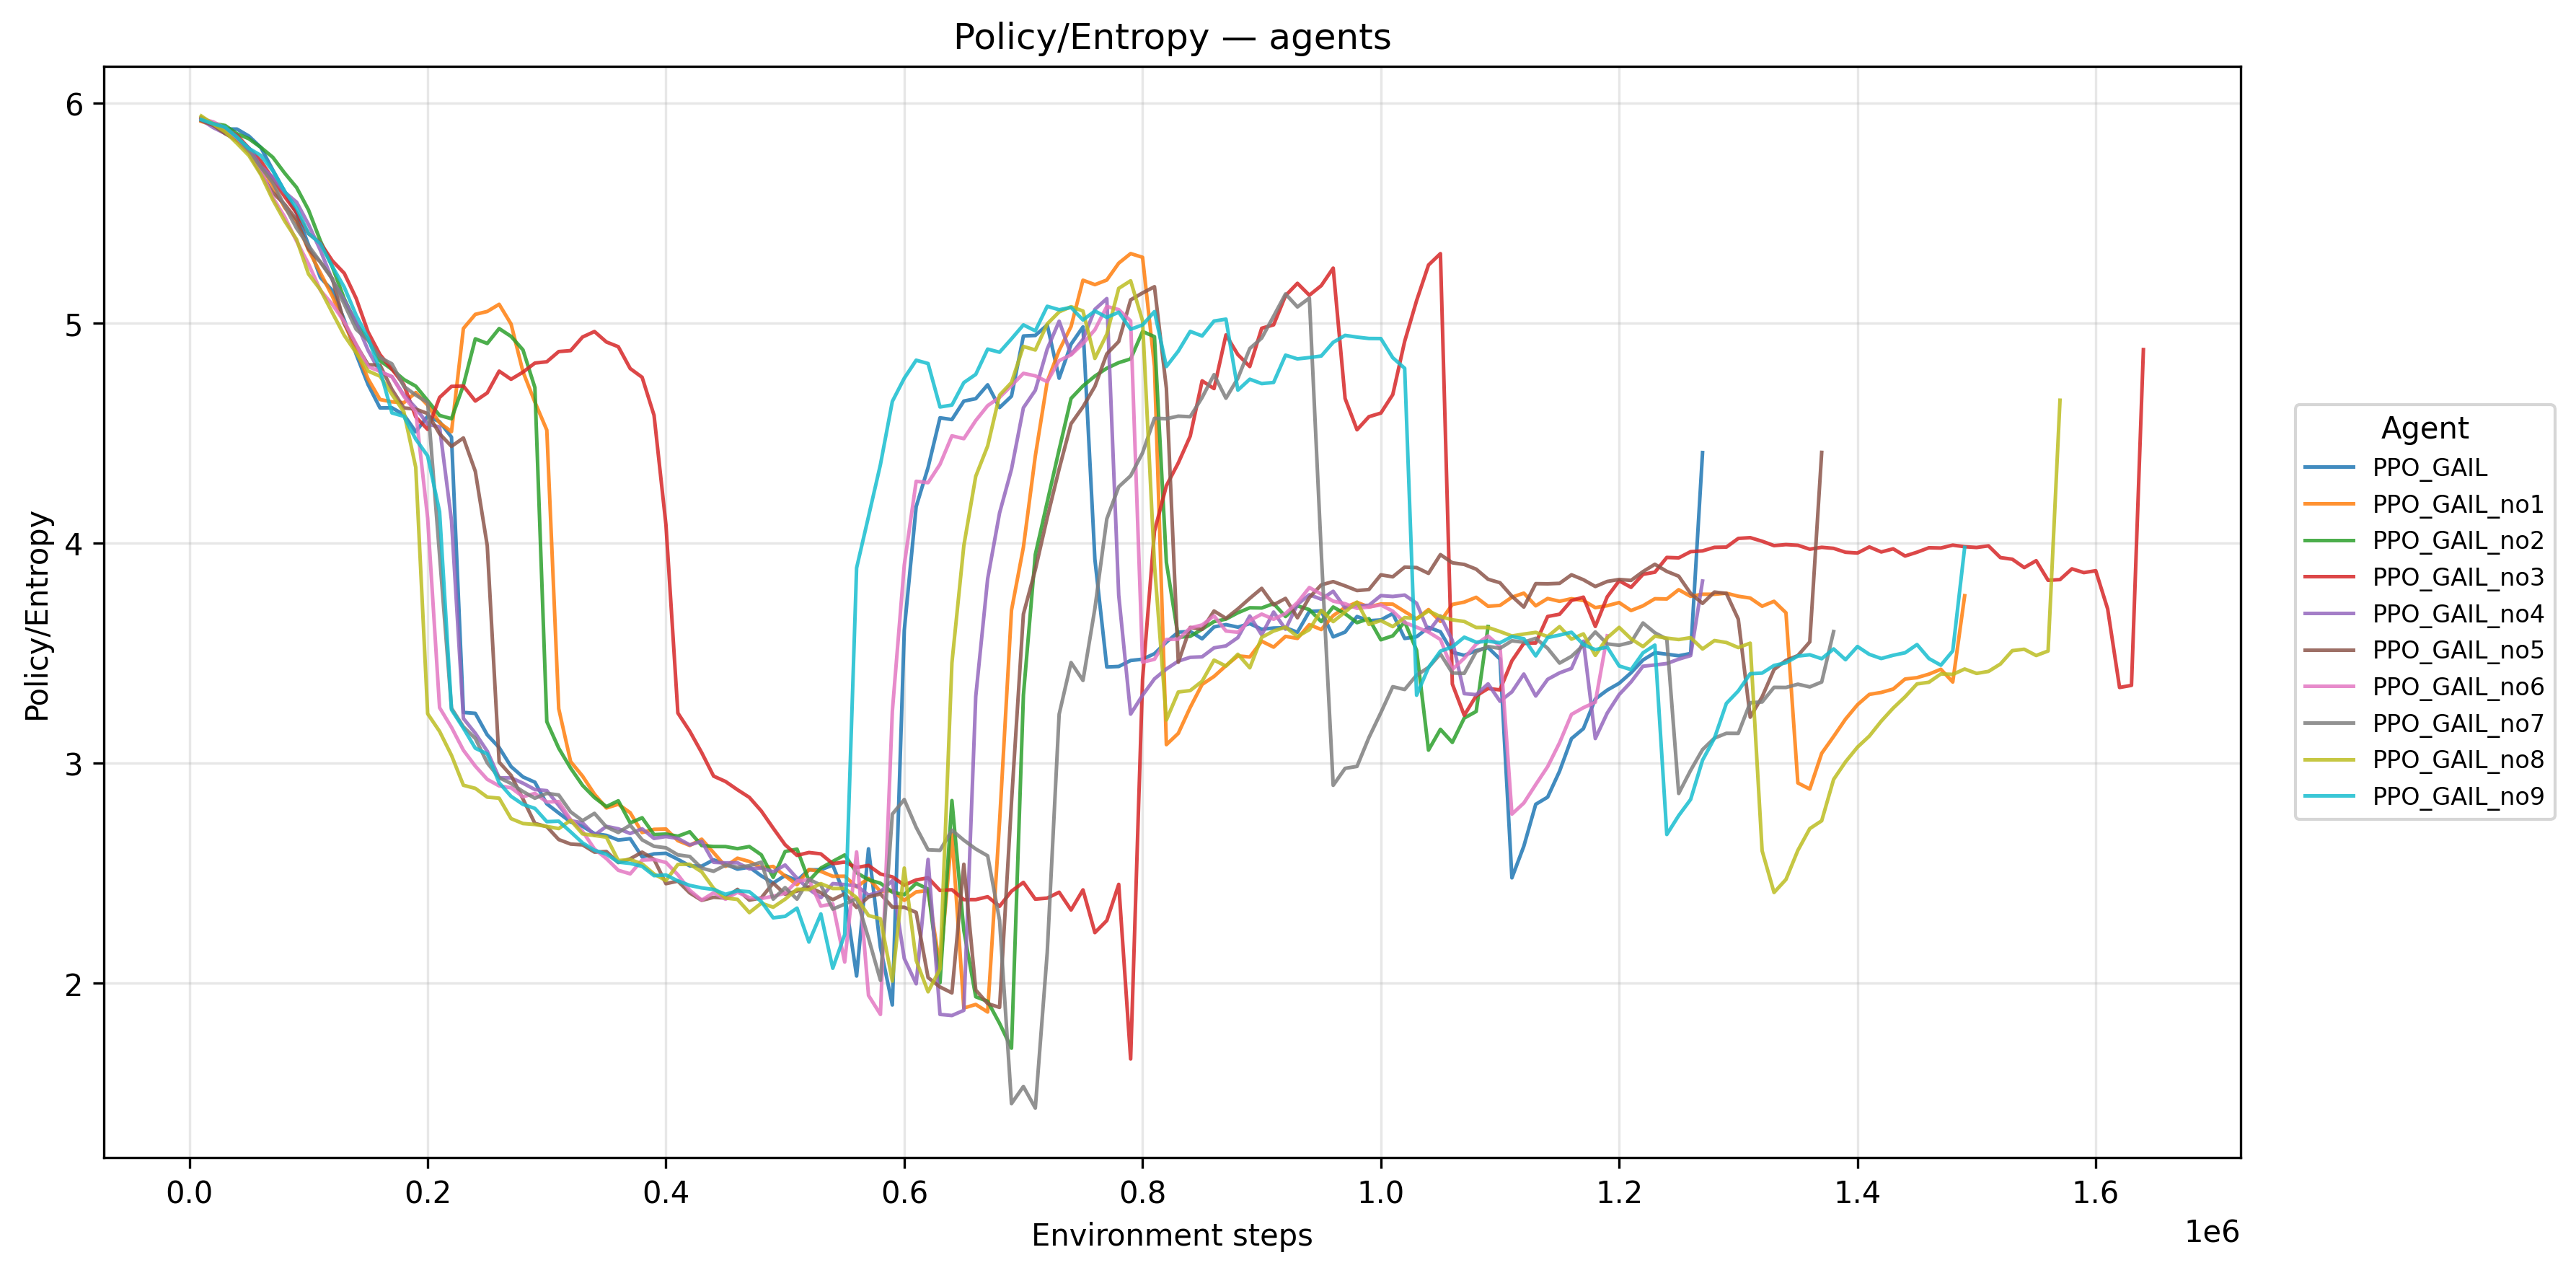
\includegraphics[width=1.0\textwidth]{images/gail_results/Policy_Entropy_agents.png}
	%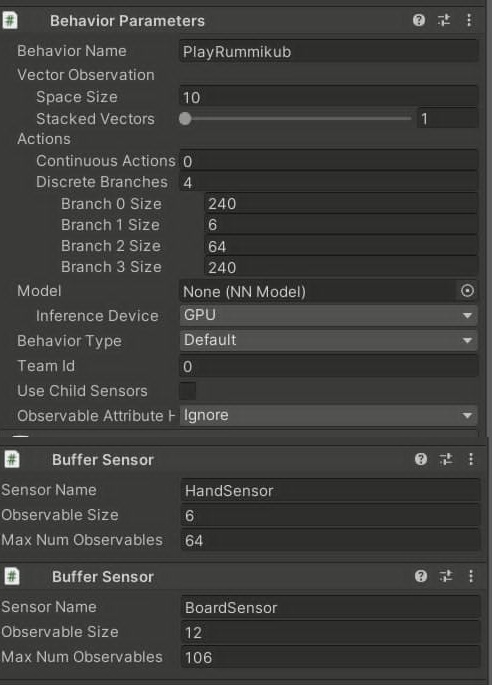
\includegraphics[width=0.7\textwidth]{images/BF_image.jpg}
	
	%	\figureplaceholder{
	%	Placeholder: GAIL entropy
	%}
	\caption{
		Entropy chart of individual 10 gail agents
	}
	\label{fig:ppo_gail_entropy}
\end{figure}


After a sudden spike, there was a sharp decline, which has now stabilized within the range of 3 to 4. Occasionally, the values have fallen below this range, but they have always returned to it. These drops and spikes are directly linked to promotions, but the fluctuations are less significant than they were initially. This may indicate a gradual stabilization of the agents' behavior. Meanwhile, the agents maintained a moderate level of exploration, enabling them to adapt their strategies to subsequent learning levels.

Agent \textit{PPO\_GAIL\_no9} experienced a significant decrease in reward around 900,000 steps, despite not receiving a promotion at that time. However, the entropy graph shows no significant change in the agent’s curve during this period. This suggests that the temporary drop in reward may have resulted from a series of more difficult or unfavorable episodes rather than a clear change in the level of exploration.

Figure \ref{fig:ppo_gail_entropy_mean_SD} summarizes the policy entropy of the PPO+GAIL agents. The mean entropy initially decreased from approximately 5.9 to 2.4, indicating that the agents gradually reduced random exploration and developed more consistent behavior while acquiring the initial curriculum skills. Around 600,000 environment steps, the entropy increased again and reached approximately 4.5, suggesting renewed exploration after the introduction of substantially more complex tasks. It subsequently stabilized mainly between 3.4 and 4.1, indicating that the agents maintained a moderate degree of exploration while adapting to the later curriculum stages.

The standard-deviation band is narrow during the initial decrease, showing similar early policy development across the training runs. It becomes considerably wider during the renewed exploration stage, indicating that individual agents responded to the increase in task difficulty at different rates. The later narrowing of the band suggests more consistent policy behavior after adaptation. The final increase should be interpreted cautiously because most agents had already completed training, leaving only a small number of active runs in the calculation.

\begin{figure}[H]
	\centering
	
	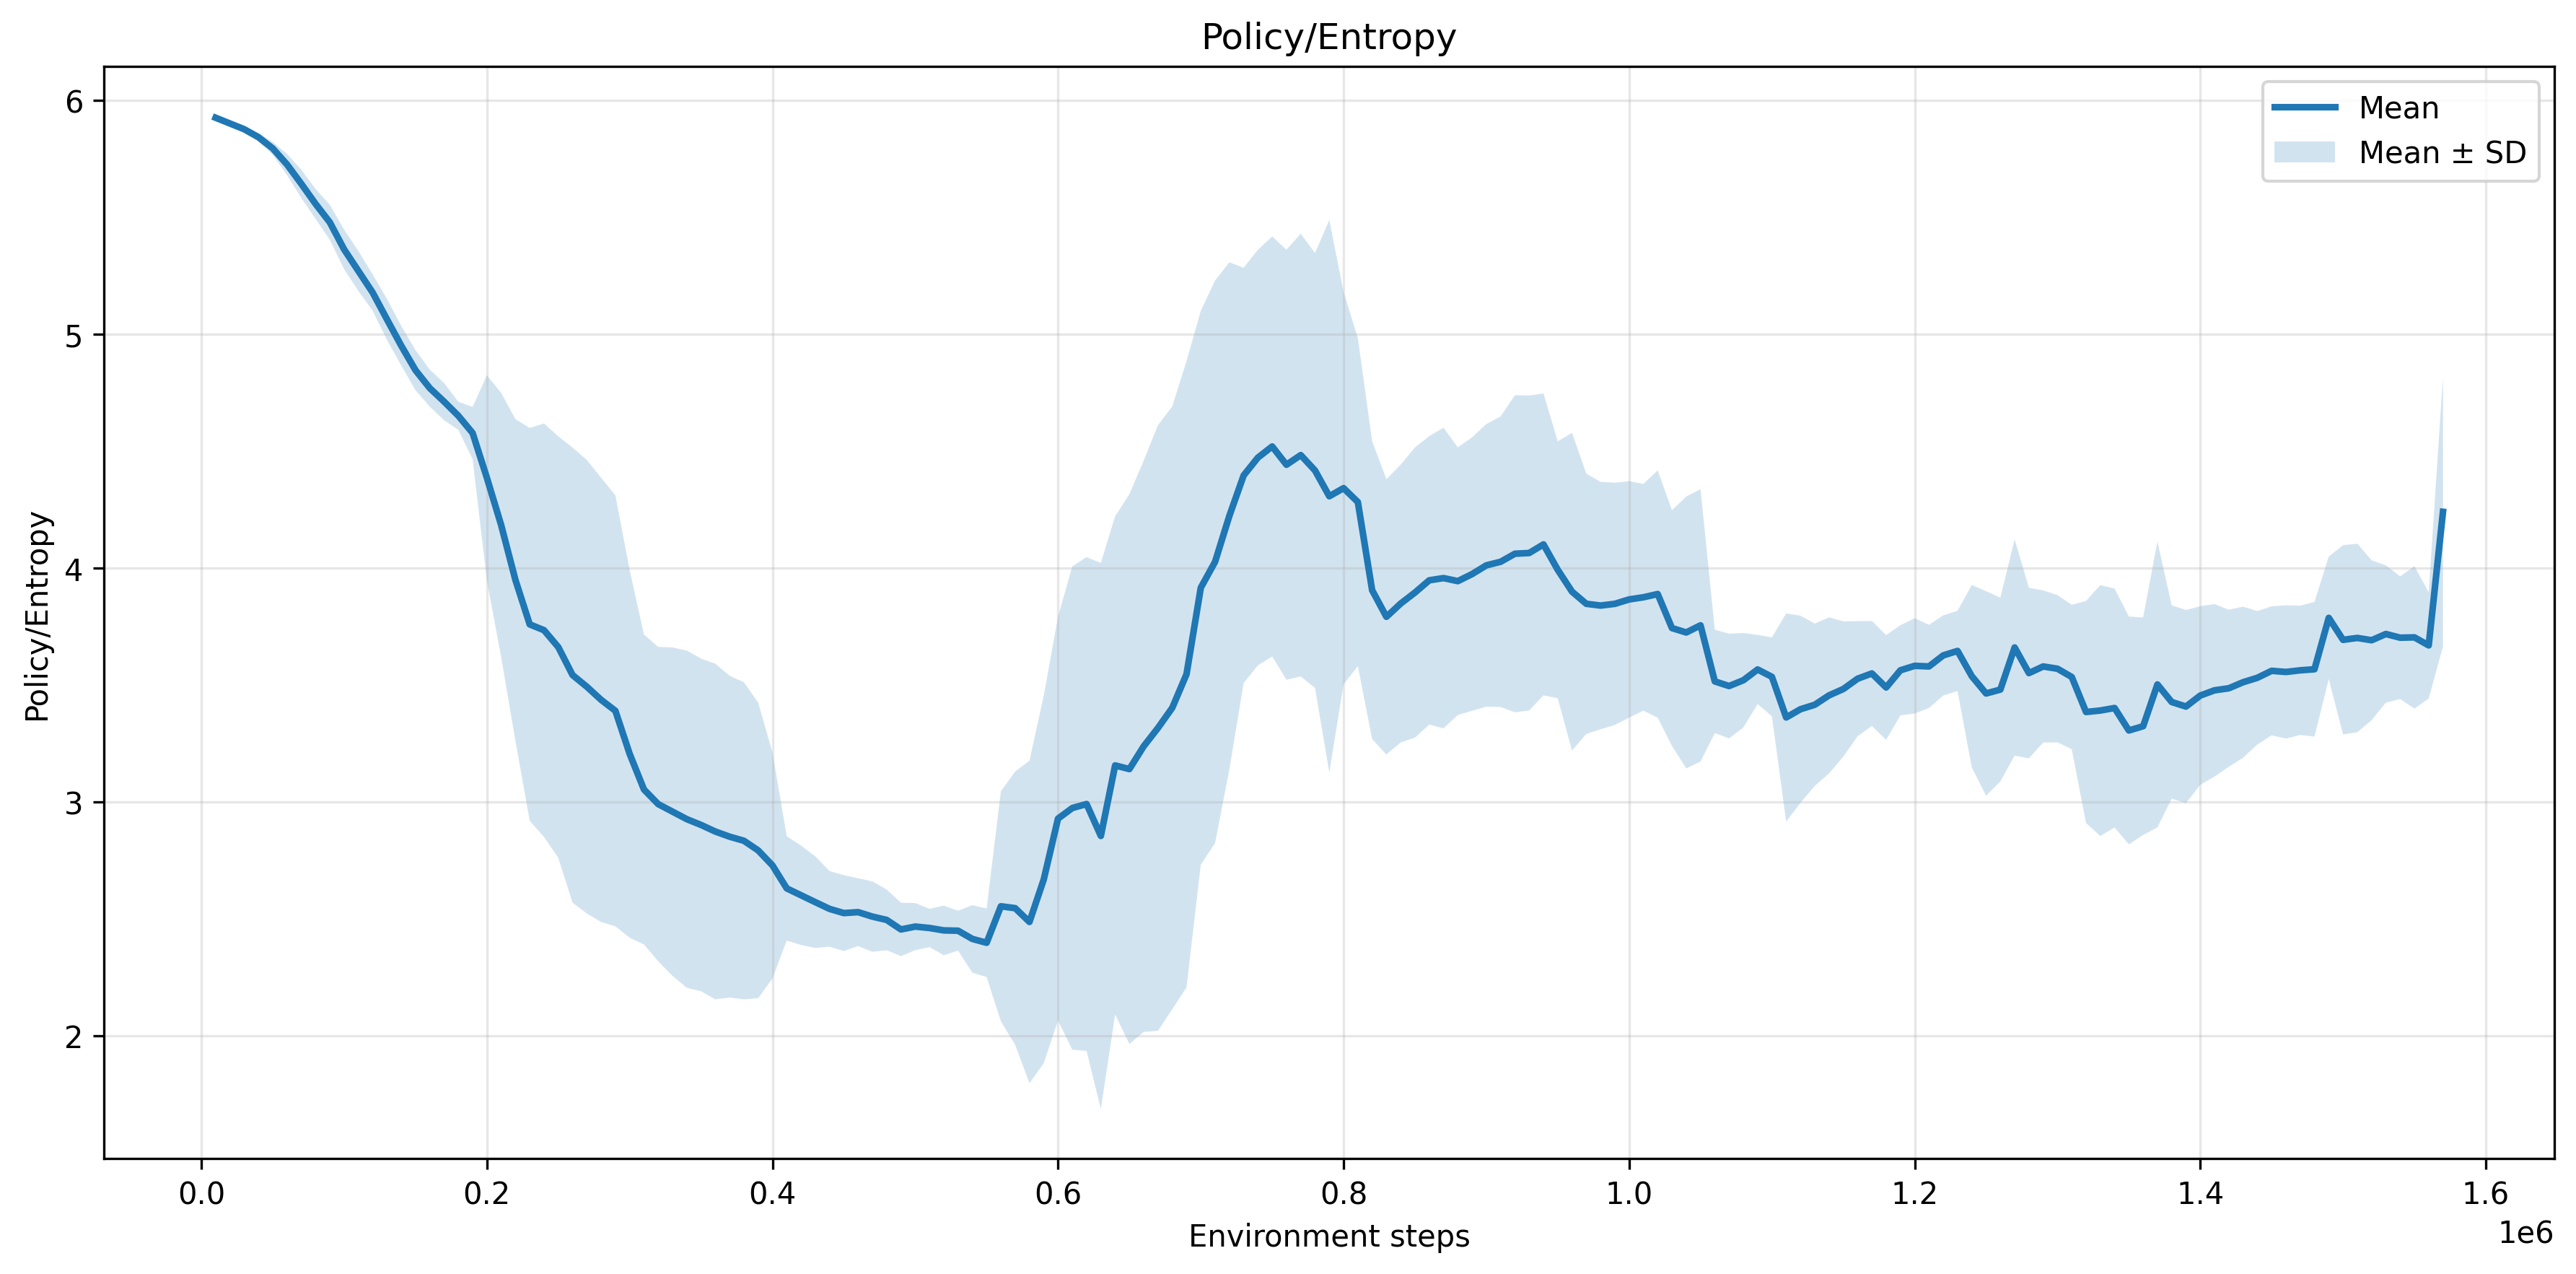
\includegraphics[width=1.0\textwidth]{images/gail_results/Policy_Entropy_mean_sd.png}
	%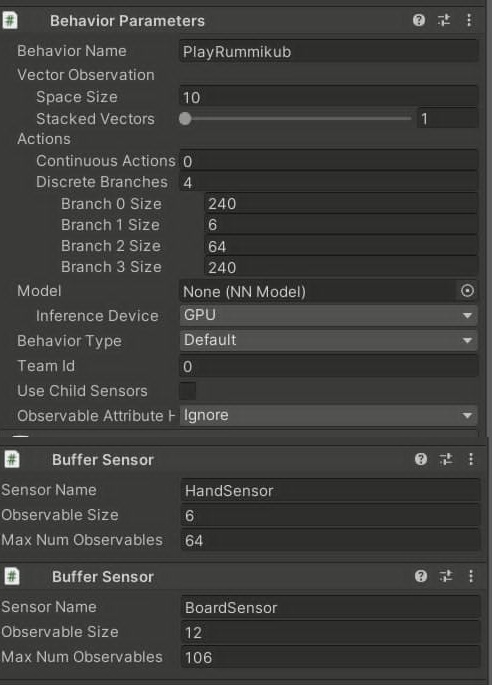
\includegraphics[width=0.7\textwidth]{images/BF_image.jpg}
	
	%	\figureplaceholder{
		%	Placeholder: GAIL entropy
		%}
	\caption{
		Entropy chart of mean and SD of individual 10 gail agents
	}
	\label{fig:ppo_gail_entropy_mean_SD}
\end{figure}



\begin{table}[H]
	\centering


		\caption{
		First recorded training steps at which individual GAIL agents completed the level.
	}
		\label{tab:gail_steps_per_level}
	\resizebox{\textwidth}{!}{%
		\begin{tabular}{
				c
				r r r r r r
				r r r r r r
			}
			\toprule
			
			\textbf{Run}
			& \textbf{L0}
			& \textbf{L1}
			& \textbf{L2}
			& \textbf{L3}
			& \textbf{L4}
			& \textbf{L5}
			& \textbf{L6}
			& \textbf{L7}
			& \textbf{L8}
			& \textbf{L9}
			& \textbf{L10}
			& \textbf{L11}
			\\
			
			\midrule
			
			0  & 220 & 550 & 570 & 580 & 580 & 580 & 590 & 590 & 600 & 760 & 1 110 & 1 270 \\
			1  & 310 & 630 & 640 & 640 & 650 & 650 & 660 & 670 & 680 & 810 & 1 340 & 1 490 \\
			2  & 290 & 620 & 640 & 650 & 650 & 650 & 660 & 690 & 700 & 820 & 1 030 & 1 090  \\
			3  & 400 & 760 & 770 & 780 & 780 & 790 & 790 & 790 & 800 & 1 060 & 1 610 & 1 640  \\
			4  & 220 & 600 & 620 & 620 & 630 & 630 & 630 & 650 & 660 & 780 & 1 180 & 1 270 \\
			5  & 250 & 610 & 650 & 650 & 660 & 660 & 660 & 680 & 690 & 820 & 1 300 & 1 370  \\
			6  & 200 & 540 & 560 & 560 & 570 & 570 & 570 & 580 & 590 & 780 & 1 090 & 1 190  \\
			7  & 210 & 570 & 590 & 590 & 680 & 690 & 700 & 720 & 720 & 950 & 1 240 & 1 380 \\
			8  & 190 & 580 & 600 & 610 & 610 & 610 & 620 & 630 & 640 & 810 & 1 320 & 1 570\\
			9  & 210 & 520 & 530 & 540 & 540 & 540 & 550 & 550 & 560 & 1 030 & 1 240 & 1 490 \\
			
			\midrule
			
			\textbf{Mean}
			& 250 & 598 & 617 & 621 & 635 & 637
			& 643 & 655 & 664 & 862 & 1246 & 1376\\
			
			\textbf{SD}
			& 62.2 & 63.8 & 62.9 & 63.8 & 64.1 & 67.1
			& 65.7 & 67.9 & 67.0 & 103.9 & 156.1 & 165.0\\
			
			\bottomrule
		\end{tabular}%
	}
	
%	\begin{minipage}{0.95\textwidth}
%		\footnotesize
%		Values are reported in thousands of environment steps. TensorBoard summaries were recorded every 10\,000 environment steps. Therefore, each value corresponds to the first recorded training step at which the given curriculum level was observed rather than the exact promotion step. A dash (--) indicates that the corresponding level was not reached during training. Mean and standard deviation were calculated only for agents that reached the corresponding curriculum level.
%	\end{minipage}
\end{table}
Values are reported in thousands of environment steps. TensorBoard summaries were recorded every 10\,000 environment steps. Therefore, each value corresponds to the first recorded training step at which the given curriculum level was observed rather than the exact promotion step. A dash (--) indicates that the corresponding level was not reached during training. Mean and standard deviation were calculated only for agents that reached the corresponding curriculum level.

The table \ref{tab:gail_steps_per_level} presents the time intervals within which each agent, using the GAIL auxiliary method, successfully completed a given level and advanced to the next one.

The first challenge was to complete Level Zero, which took an average of 250,000 steps, a task that may involve learning to map observations to one’s actions.
Agent \textit{PPO\_GAIL\_no8} took the least time to complete this level, advancing after 190,000 steps. In contrast \textit{PPO\_GAIL\_no3} did not advance until after 400,000 steps, which makes it a difference of 210,000 steps.

Level 1 proved to be another challenge. On average, agents reached this level after 250,000 steps and completed it after 598,000 steps, which means it took an average of 248,000 steps to complete Level 1. However, at this level, the agent \textit{PPO\_GAIL\_no9} performed the best, advancing after 520,000 steps. Between its advancement from level zero, which occurred after 210,000 steps, it took approximately 310 steps to reach level two.

Completing levels 2-–8 required fewer steps, as can also be seen in Figure \ref{fig:gail_lessonNumber}. The agents completed level 1 after 598,000 steps and level 8 after an average of 664,000 steps, which means that the agents successfully completed levels 2 through 8 in an average of 66,000 steps. This suggests that the given set of tasks was similar enough to the previous levels that, after mastering tasks 0 and 1, the agents could quickly adapt to levels 2–-8.

Level 9 proved to be a greater challenge for the agents. On average, advancing from level 9 to 10 required 198,000 steps. The first agent to complete level 9 was \textit{PPO\_GAIL}, who advanced to level 10 after 760,000 steps. However, the agent \textit{PPO\_GAIL\_no3} advanced the latest, reaching level 10 after 1.06 million steps, which means that the difference between the time of advancement for agent \textit{PPO\_GAIL} and agent \textit{PPO\_GAIL\_no3} is 300,000 steps. However, agent \textit{PPO\_GAIL\_no9} took the longest to complete Level 9. He completed level 8 after 560,000 steps, but finished level 9 after 1.03 million steps, which shows that it needed 470,000 steps to complete the level.

Level 10 turned out to be the most time-consuming for agents on average, as they completed this level after 1.246 million steps on average, meaning that agents needed an average of 384,000 steps after completing Level 9. Agent \textit{PPO\_GAIL\_no2} performed best at this stage, completing Level 10 after 1.03 million steps. Agent \textit{PPO\_GAIL\_no9} also completed this level relatively quickly, after 210,000 steps. In contrast, agents \textit{PPO\_GAIL\_no1}, \textit{PPO\_GAIL\_no3}, and \textit{PPO\_GAIL\_no8} required over 500,000 steps to meet the promotion criteria.

Reaching the target level was faster, as it took an average of 130,000 steps between levels. However, the time it took to complete Level 11 varied among the agents. Agent \textit{PPO\_GAIL\_no3} needed only 30,000 steps to meet the promotion requirements, and agent \textit{PPO\_GAIL\_no2} required 60,000 steps. In contrast, agents \textit{PPO\_GAIL\_no8} and \textit{PPO\_GAIL\_no9} required as many as 250,000 steps to meet the promotion criteria.

Throughout the learning process, the standard deviation increases as the curriculum progresses. Initially, the standard deviation is very similar, as are the values across levels 2–-8, where agents advanced quickly. However, the greatest differences appear at levels 9-11, with the highest value occurring at level 11. This result may not only be due to the length of study at level 11, but also to varying delays in studying the previous levels.

While all agents achieved the set training goal, the pace of their progress varied greatly. Levels 0, 1, 9 and 10 were the most demanding in terms of the number of steps required, with level 10 taking the most time on average. Levels 2–8 were completed quickly, possibly indicating the transfer of previously acquired skills.
\begin{table}[htbp]
	\centering
	\caption{
		Training outcome of individual PPO GAIL agents.
	}
	\label{tab:gail_training_time}
	
	\begin{tabular}{c c c c}
		\toprule
		
		\textbf{Agent}
		&
		\textbf{Training stopped at step}
		&
		\textbf{Target reached}
		&
		\textbf{Training time [h]}
		\\
		
		\midrule
		
		0  & 1270 & Yes & 12.78 \\
		1  & 1490 & Yes & 10.97 \\
		2  & 1090 & Yes & 10.13 \\
		3  & 1640 & Yes & 13.32 \\
		4  & 1270 & Yes & 9.31 \\
		5  & 1370 & Yes & 9.76 \\
		6  & 1190 & Yes & 8.43 \\
		7  & 1380 & Yes & 10.88 \\
		8  & 1570 & Yes & 10.62 \\
		9  & 1490 & Yes & 10.98\\
		
		\midrule
		
		\textbf{Mean}
		&
		1376
		&
		100\%
		&
		10.7 \\
		
		\textbf{SD}
		&
		165.0
		&
		
		&
		1.40 \\
		
		\bottomrule
	\end{tabular}
	
	%	\begin{minipage}{0.95\textwidth}
	%	\footnotesize
	%	Values in the second column are reported in thousands of environment steps and correspond to the first TensorBoard summary in which level 12 was observed.
	%\end{minipage}
\end{table}
Values in the second column are reported in thousands of environment steps and correspond to the first TensorBoard summary in which level 12 was observed.

The table \ref{tab:gail_training_time} displays the success rate in reaching the goal, the number of steps required, and how long it took each agent to complete the training.

The target effectiveness is 100\%, which means that every agent using the GAIL auxiliary method reaches the target level.

In terms of the number of steps taken, the most efficient agent was \textit{PPO\_GAIL\_no2}, which completed training after 1.09 million steps. By contrast, \textit{PPO\_GAIL\_no3} took the longest, performing 1.64 million steps before reaching the goal. This difference of 550,000 steps shows that identical hyperparameters do not lead to an identical training process.

The average training time was 10.7 hours, with a standard deviation of 1.4 hours. However, the most time-efficient agent was \textit{PPO\_GAIL\_no6}, which reached the goal after 8.43 hours, even though it completed 1.19 million steps during training. Agent \textit{PPO\_GAIL\_no3} took the longest to learn, at 13.32 hours. The difference between the most efficient and least efficient times is as much as 4.89 hours.

The results of agents \textit{PPO\_GAIL} and \textit{PPO\_GAIL\_no4} are striking. On average, they finished training at similar times, but the \textit{PPO\_GAIL} agent completed training after 12.78 hours, while \textit{PPO\_GAIL\_no4} finished training after just 9.31 hours. 
%It appears that despite similar results and the number of steps, agent \textit{PPO\_GAIL\_no4} processed data more efficiently during training.

Overall, the duration of the learning process was influenced not only by the number of steps in the environment required to achieve the goal. The instantaneous load on the device’s components, the complexity of the episodes, and data logging to TensorBoard also had a significant impact. In the case of the GAIL auxiliary method, the additional imitation signal and discriminator updates may have also contributed to the computational cost.
The table shows that GAIL achieved 100\% effectiveness in accomplishing the set goal, but the number of steps and training time varied significantly. The \textit{PPO\_GAIL\_no2} agent was the most efficient in terms of the number of trials, while the \textit{PPO\_GAIL\_no6} agent was the most efficient in terms of elapsed time. The lack of a strict proportionality between steps and hours indicates significant differences in the computational throughput between individual runs.
\subsubsection{Evaluation results}
The table \ref{tab:gail_evaluation_results} presents the test results of ten GAIL agents trained at level eleven.
\begin{table}[H]
	\centering
	\caption{Evaluation results of PPO GAIL agents over 1000 episodes on curriculum level 11.}
	\label{tab:gail_evaluation_results}
	\begin{tabular}{c r r r r}
		\toprule
		\textbf{Agent} &
		\textbf{Episodes} &
		\textbf{Wins} &
		\textbf{Losses} &
		\textbf{Win rate [\%]} \\
		\midrule
		0 & 1000 & 731 & 269 & 73.1 \\
		1 & 1000 & 701 & 299 & 70.1 \\
		2 & 1000 & 724 & 276 & 72.4 \\
		3 & 1000 & 739 & 261 & 73.9 \\
		4 & 1000 & 709 & 291 & 70.9 \\
		5 & 1000 & 709 & 291 & 70.9 \\
		6 & 1000 & 684 & 316 & 68.4 \\
		7 & 1000 & 700 & 300 & 70.0 \\
		8 & 1000 & 624 & 376 & 62.4 \\
		9 & 1000 & 677 & 323 & 67.7 \\
		\midrule
		\textbf{Total} &
		\textbf{10\,000} &
		\textbf{6998} &
		\textbf{3002} &
		\textbf{} \\
		\textbf{Mean} &
		&
		&
		&
		69.98 \\
		\textbf{SD} &
		&
		&
		&
		3.1 \\
		\bottomrule
	\end{tabular}
\end{table}
Each agent was tested over 1,000 episodes, for a total of 10,000 episodes across the entire evaluation. The agents collectively achieved 6,998 wins and 3,002 losses, resulting in an overall success rate of 69.98\%.

Agent \textit{PPO\_GAIL\_no3} achieved the best result, with a score of 73.9\%, but the results do not differ significantly from those of the other agents, the second-best agent, \textit{PPO\_GAIL\_no2}, scored 72.4\%. This shows that despite a significantly longer training time, agent \textit{PPO\_GAIL\_no3} achieved very similar results.

Agent \textit{PPO\_GAIL\_no8} performed the worst, achieving a score of 62.4\%. The difference between the best and worst results is as much as 11.5 percentage points. This is a significant discrepancy, given that the agents’ configurations were identical. Achieving the same training goal did not, therefore, lead to identical final performance, and the number of steps required to advance was not a clear predictor of the subsequent evaluation result.
\subsection{Cross-model comparison}

The table \ref{tab:cross_model_level_comparison} presents a summary of the average completion times for each level of the curriculum, the standard deviation, and the difference between them. The average scores were calculated among agents who completed a given level.
\begin{table}[H]
	\centering
	\caption{Comparison of curriculum-level completion and transition times
		for PPO baseline and PPO+GAIL agents.}
	\label{tab:cross_model_level_comparison}
	\scriptsize
	\setlength{\tabcolsep}{5pt}
	
	\begin{tabular}{c rrr rrr rr}
		\toprule
		& \multicolumn{3}{c}{PPO Baseline}
		& \multicolumn{3}{c}{PPO+GAIL}
		& \multicolumn{2}{c}{Difference} \\
		\cmidrule(lr){2-4}
		\cmidrule(lr){5-7}
		\cmidrule(lr){8-9}
		Level
		& Completion & SD & Transition
		& Completion & SD & Transition
		& Completion & Transition \\
		\midrule
		L0  & 216.0  & 41.0  & 216.0
		& 250.0  & 62.2  & 250.0
		& +34.0  & +34.0 \\
		
		L1  & 556.7  & 50.5  & 340,7
		& 598.0  & 63.8  & 348.0
		& +41.3  & +7.3 \\
		
		L2  & 578.9  & 49.5  & 22.2
		& 617.0  & 62.9  & 19.0
		& +38.1  & -3.2 \\
		
		L3  & 578.9  & 49.5  & <1.0
		& 621.0  & 63.8  & 4.0
		& +42.1  & >+3 \\
		
		L4  & 588.9  & 49.5  & 10.0
		& 635.0  & 64.1  & 14.0
		& +46.1  & +4.0 \\
		
		L5  & 588.9  & 49.5  & <1.0
		& 637.0  & 67.1  & 2.0
		& +48.1  & >+1.0 \\
		
		L6  & 588.9  & 49.5  & <1.0
		& 643.0  & 65.7  & 6.0
		& +54.1  & >+5 \\
		
		L7  & 605.6  & 46.7  &  16.7
		& 655.0  & 67.9  & 12.0
		& +49.4  & -4.7 \\
		
		L8  & 611.1  & 48.1  & 5.5
		& 664.0  & 67.0  & 9.0
		& +52.9  & +3.5 \\
		
		L9  & 798.9  & 74.4  & 187.8
		& 862.0  & 103.9 & 198.0
		& +63.1  & +10.2 \\ 
		
		L10 & 1096.7 & 101.5 & 297.8
		& 1246.0 & 156.1 & 384.0
		& +149.3 & +86.2 \\ 
		
		L11 & 1274.4 & 183.9 & 177,7
		& 1376.0 & 165.0 & 130
		& +101.6 & -47,7 \\
		\bottomrule
	\end{tabular}
	
	\vspace{0.2cm}
	%\begin{minipage}{0.98\textwidth}
	%	\footnotesize
	%	Values are reported in thousands of environment steps.
	%	\textit{Completion} denotes the first recorded training step at
	%	which the corresponding level was completed.
	%	\textit{Transition} denotes the mean number of steps required to
	%	complete the level after entering it. Positive differences indicate
	%	larger values for PPO+GAIL. Transition statistics were calculated
	%	only from agents that completed both boundaries of the corresponding
	%	transition.
	%\end{minipage}
\end{table}
	Values are reported in thousands of environment steps. \textit{Completion} denotes the first recorded training step at which the corresponding level was completed. \textit{Transition} denotes the mean number of steps required to complete the level after entering it. Positive differences indicate larger values for PPO+GAIL. Transition statistics were calculated only from agents that completed both boundaries of the corresponding transition.

It is important to note that the results include averages for agents who reached each level. For levels 1–11, the baseline average is calculated from nine agents, whereas for the GAIL models, it is calculated from ten agents.
Among the agents that completed the analysed levels, the PPO Baseline recorded an average of fewer cumulative steps to complete each level. However, the differences in time taken to complete individual levels were inconsistent.

Level zero was the first time-consuming training stage for both models, but it posed greater difficulties for the GAIL model, with a difference of 34,000 steps between the models. The results suggest that incorporating GAIL did not accelerate the initial task in the curriculum. PPO+GAIL agents required more training and had more variable completion times for the level.

Level one already required a relatively similar amount of time, as the average difference between the two models was only 7,300. It can therefore be concluded that this level posed a similarly significant challenge for both methods, although PPO+GAIL required slightly more training time on average.
In order to complete Level 2, the baseline required an additional 3,200 steps. However, this is a minor difference compared to the total number of steps required so far.

At levels 3–8, both configurations made rapid progress, and the transitions often occurred within a single TensorBoard recording interval. Although they reached these levels at different times, both models achieved them after a similar number of steps. This may indicate that tasks 3–8 were relatively easy to master once the models had acquired the necessary skills, or that they largely relied on behaviors learned in previous levels. 

Level nine presented another bottleneck for both models. For the baseline model, the transition took an average of 187,800 steps, while for the model using the GAIL auxiliary method, it took an average of 198,000 steps. The difference of 10,200 steps was small relative to the total number of steps required at this level.

Level 10 shows the greatest difference between the models. The baseline model completed Level 10 after approximately 297,800 steps, while the GAIL model completed it after approximately 384,000 steps. The average difference between the models is as high as approximately 86,200 steps, which is the largest difference in the average time to complete a single level.

Level 11, indicating the achievement of the learning goal, showed that the GAIL agents performed better at this stage, requiring approximately 47,700 fewer steps than the baseline agents. However, in the final analysis, the baseline agents required fewer steps overall, as they successfully completed training after an average of 1,274,400 steps, while the GAIL model required an average of 1,376,000. However, it should be noted that the final results for the baseline included only agents that had learned Level 11. The difference in the number of steps to complete Level 11 is 101,600, which is not a significant difference over the course of the entire training. Given the use of expert demonstrations, it was assumed that the additional GAIL signal might reduce the number of steps needed to master the tasks. The results did not confirm this assumption with respect to the entire curriculum analyzed.

PPO+GAIL did not accelerate the achievement of the overall goal. Both configurations progressed through L1–L9 at a similar pace. PPO+GAIL’s main loss occurred at L10 and some of this was offset at L11. However, the speed comparison only applies to successful runs. Meanwhile, nine out of ten Baseline agents and all PPO+GAIL agents achieved the goal.

The table \ref{tab:cross_model_training} presents a summary of the results for both RL models, including training reliability, training cost, and final policy quality. In the analyzed sample, all ten PPO+GAIL agents and nine out of ten PPO Baseline agents achieved the objective. This means that PPO+GAIL demonstrated greater observed reliability across all trained agents.

The average number of steps to termination is 1,347,000 for the PPO baseline, and 1,376,000 steps for the PPO GAIL agent, a difference of only 29,000 steps. However, this result for the baseline is the average of the results of all agents, including the \textit{PPO\_baseline\_no1} agent, which terminated training after 2 million steps because it failed to reach the final goal within the specified time. Considering only the agents that reached the specified goal, this average is 1,274,400 steps, resulting in a difference of 101,600 steps between the models. For all agents, runs stopped on average at a similar number of steps, however, for the agents that reached the goal, the baseline model required fewer steps on average.

\begin{table}[H]
	\centering
	\caption{Comparison of curriculum training outcomes.}
	\label{tab:cross_model_training}
	\begin{tabular}{l c c c}
		\toprule
		\textbf{Metric} &
		\textbf{baseline all} &
		\textbf{baseline successful} &
		\textbf{PPO + GAIL} \\
		\midrule
		Agents reaching the target  & 9/10 & - & 10/10 \\
		Mean stopping step          & 1347 & 1274,4 & 1376 \\
		SD of steps                 & 278.96 & 183,9 & 165.0 \\
		Mean training time [h]      & 5.12 & 4,67 &10.7 \\
		SD of training time [h]     & 1.5 & 0.71 &1.4 \\
		Evaluation mean [\%] 			& 65.09 &68,39  & 69.98\\
		Evaluation SD [\%]			& 10.26	& 2.83 &3.1 \\
		Evaluation max result [\%] 		& 72.1	& 72.1 &73.1\\
		Evaluation min result [\%] 		& 35.3	& 63.1	&62.4\\
		\bottomrule
	\end{tabular}
\end{table}


The standard deviation of 278.96 thousand for the baseline also takes into account the agent that failed to achieve the intended goal. However, when considering only the successful agents, the standard deviation of the baseline model is 183.9 thousand steps, which is still greater than that of the GAIL model, whose standard deviation is 165 thousand steps.

The average training time varies significantly across models. The baseline model required an average of 5.12 hours, while the GAIL model required an average of 10.7 hours, representing a computational demand that is twice as high. This result may be directly attributable to the computational cost of updating the discriminator and processing demonstrations, as well as differences in device load.

The final evaluation of both models shows an accuracy of 65.09\% and a standard deviation of 10.26 for the baseline model, and an accuracy of 69.98\% and a standard deviation of 3.1 for the GAIL model. This shows that, ultimately, agents trained using the GAIL auxiliary method achieved a result that was nearly 5\% better in the environment. However, for the baseline model, these results include an ineffective agent, when considering only agents that successfully completed training, the average is 68.39\% with a standard deviation of 2.83. This means that when considering only effective agents, the effectiveness of the models’ policies is very similar.

The minimum and maximum evaluation results further demonstrate the influence of the unsuccessful baseline agent. When all baseline agents are considered, the observed win rates range from 35.3\% to 72.1\%. After excluding the agent that failed to reach the training target, the minimum increases to 63.1\%, while the maximum remains unchanged at 72.1\%. The successful baseline agents therefore cover a range of 9.0 percentage points. The PPO+GAIL results range from 62.4\% to 73.1\%, corresponding to a range of 10.7 percentage points. Thus, after restricting the comparison to successfully trained policies, the extreme evaluation results of both methods are similar, with PPO+GAIL achieving a slightly higher maximum and PPO Baseline a slightly higher minimum.

\section{Conclusions}

Both configurations demonstrated the ability to learn the tasks defined in the curriculum. Most of the baseline agents and all of the GAIL agents reached the target level, which was completing Level 11.

However, this did not mean that the task had been fully mastered. During the evaluation, both methods achieved results in the range of 65\%–70\%. The criterion for curriculum advancement was therefore not equivalent to 100\% reliability of the policy.

The overall progression structure was similar for both models. Both models required more steps at Level 0, which involved mastering the basics of the environment’s mechanics. Level 1 also proved to be the first challenge, followed by rapid progression between levels 2 and 8, which may indicate that the skills acquired in the first two levels were transferable to subsequent tasks. For both models, level 9 marked a renewed increase in difficulty, and level 10 proved to be the most difficult.

In both configurations, the reward initially rose from strongly negative values to values close to zero or positive. Most of the sharp drops could be linked to a change in the curriculum level. Therefore, they did not automatically indicate PPO instability. There were also isolated exceptions. For example, a large drop in agent \textit{PPO\_GAIL\_no9} occurred without a promotion. This can be described as a short-term deterioration in performance or an isolated fluctuation. Since the agent later recovered its reward and continued its progression, this was not a permanent breakdown in the learning process.

The entropy of both configurations exhibited a cyclical pattern, initially reaching high values, then decreasing as the task was mastered, and subsequently increasing upon reaching a new level. Later in the training, the entropy of most agents remained mainly between 3 and 4, and its fluctuations were smaller. This indicates a relative stabilization of the exploration level, subsequent updates no longer caused such large changes in the diversity of selected actions. The most notable case was the unsuccessful \textit{PPO\_baseline\_no1}, whose entropy dropped rapidly and remained significantly lower than that of the other agents for a long time. This may suggest premature convergence to an ineffective strategy.

The scope of the acquired behavior should be distinguished from mastery of the full Rummikub game. The curriculum examined selected tile-placement skills in a controlled, single-agent environment, with no opponents or turn-time limit. These skills included completing and independently creating runs and groups, selecting suitable placements for multiple tiles, identifying different arrangement types and making decisions when faced with additional arrangements on the board. Consequently, the results demonstrate the agents' ability to acquire these particular rule-based placement skills, rather than a complete multiplayer Rummikub strategy.

The results suggest that acquiring a new skill depends not only on the number of required actions, but also on the type of change introduced to the task. When a level involved extending a previously learned behavior by requiring more tiles to be placed under similar conditions, the agents generally progressed quickly. This indicates that representations and action patterns acquired in earlier tasks can be transferred to more demanding variants. However, introducing qualitatively different decision problems, such as selecting actions in the presence of multiple arrangements, resulted in longer transition periods, even when the number of additional moves remained unchanged.

Therefore, when a curriculum introduces a substantial qualitative increase in difficulty, a temporary decrease in reward can be expected, alongside renewed growth in policy entropy and greater variation between training runs. This behavior does not necessarily indicate algorithmic instability. If it coincides with a curriculum transition and is followed by reward recovery and further progression, it is more accurately understood as a period of renewed exploration and adaptation. However, a sharp deterioration that occurs without a task transition, particularly if the policy does not subsequently recover, provides stronger evidence of unstable learning or convergence to an ineffective strategy.

%This observation has implications for the design of Curriculum Learning environments. Consecutive tasks should introduce sufficiently small changes to allow previously acquired behavior to remain useful. If a new task simultaneously modifies the required arrangement, available action types, relevant board area and number of interacting elements, the resulting transition may be too large for reliable knowledge transfer. Additional intermediate lessons may then be required to separate the acquisition of new mechanics from an increase in the number of actions needed to complete the task.

The results also show that meeting a curriculum promotion threshold should be considered evidence of achieving the required level of average training performance, rather than full mastery of the relevant skill. Evaluation win rates below 100\% demonstrate that a policy may satisfy the advancement condition while failing in a considerable proportion of independently generated episodes.

The PPO Baseline configuration appears to be more appropriate when the environment can provide informative intermediate rewards, when action masking can limit invalid decisions, and when the required behaviour can be divided into gradual curriculum stages. Under these conditions, independent exploration was sufficient for most agents to acquire the desired skills while avoiding the additional computational cost of imitation learning. Therefore, this configuration is preferable when training time and computational efficiency are the primary constraints.

PPO+GAIL may be more appropriate in situations where successful exploration is challenging, representative expert demonstrations are available, or reducing the likelihood of unsuccessful training runs is more important than minimising computational cost. In the analysed sample, GAIL did not accelerate curriculum completion or produce a clear improvement in the evaluation results of successfully trained policies. However, all ten PPO+GAIL agents reached the target. This suggests that the auxiliary imitation signal may improve consistency in reaching the training objective, even when it does not improve sampling efficiency.

The effectiveness of GAIL is likely to depend on how closely the demonstrations correspond to the skills being trained. In this study, the demonstrations were recorded during full-game behaviour, whereas the training used isolated curriculum tasks. Therefore, the demonstrations may contain uncommon or unavailable states and actions in individual curriculum stages. Creating demonstrations specifically for the relevant skill categories could provide a more informative imitation signal. However, this possibility requires separate experimental verification.

Overall, PPO Baseline provided the more computationally efficient solution for learning the selected tile-placement skills, whereas PPO+GAIL provided greater observed reliability of reaching the curriculum target at the cost of substantially longer training. The results do not suggest that either configuration is universally superior. PPO Baseline is preferable when reward shaping, action masking and gradual curriculum progression already make exploration feasible. PPO+GAIL is more justified when appropriate demonstrations are available and the priority is to increase training consistency in a difficult exploration problem, provided that the additional computational cost is acceptable.
%The GAIL auxiliary method did not reduce the number of steps required to successfully train the agents. The baseline and GAIL models showed similar requirements for the number of observations, while the GAIL agents required twice as many hours of training time. This difference in training time was not due to the number of training steps required, but rather to the operation of the discriminator, the calculation of the imitation signal, and the processing of demonstrations. The evaluation results did not show that GAIL significantly improved the effectiveness of the final policy of the trained agents.

%The Baseline PPO was more efficient in terms of the number of steps and computation time among successful runs. Adding GAIL did not improve overall sampling efficiency nor did it result in a significant increase in the policies’ final effectiveness. However, in the analyzed sample, it increased the consistency of achieving the goal, at the cost of significantly longer computation time. 
%
%\begin{itemize}
%\item presentation of results, analysis and wide discussion of elaborated results, conclusions
%\end{itemize}
%
%
%
%\begin{table}
%\centering
%\caption{A caption of a table is ABOVE it.}
%\label{id:tab:wyniki}
%\begin{tabular}{rrrrrrrr}
%\toprule
%	         &                                     \multicolumn{7}{c}{method}                                      \\
%	         \cmidrule{2-8}
%	         &         &         &        \multicolumn{3}{c}{alg. 3}        & \multicolumn{2}{c}{alg. 4, $\gamma = 2$} \\
%	         \cmidrule(r){4-6}\cmidrule(r){7-8}
%	$\zeta$ &     alg. 1 &   alg. 2 & $\alpha= 1.5$ & $\alpha= 2$ & $\alpha= 3$ &   $\beta = 0.1$  &   $\beta = -0.1$ \\
%\midrule
%	       0 &  8.3250 & 1.45305 &       7.5791 &    14.8517 &    20.0028 & 1.16396 &                       1.1365 \\
%	       5 &  0.6111 & 2.27126 &       6.9952 &    13.8560 &    18.6064 & 1.18659 &                       1.1630 \\
%	      10 & 11.6126 & 2.69218 &       6.2520 &    12.5202 &    16.8278 & 1.23180 &                       1.2045 \\
%	      15 &  0.5665 & 2.95046 &       5.7753 &    11.4588 &    15.4837 & 1.25131 &                       1.2614 \\
%	      20 & 15.8728 & 3.07225 &       5.3071 &    10.3935 &    13.8738 & 1.25307 &                       1.2217 \\
%	      25 &  0.9791 & 3.19034 &       5.4575 &     9.9533 &    13.0721 & 1.27104 &                       1.2640 \\
%	      30 &  2.0228 & 3.27474 &       5.7461 &     9.7164 &    12.2637 & 1.33404 &                       1.3209 \\
%	      35 & 13.4210 & 3.36086 &       6.6735 &    10.0442 &    12.0270 & 1.35385 &                       1.3059 \\
%	      40 & 13.2226 & 3.36420 &       7.7248 &    10.4495 &    12.0379 & 1.34919 &                       1.2768 \\
%	      45 & 12.8445 & 3.47436 &       8.5539 &    10.8552 &    12.2773 & 1.42303 &                       1.4362 \\
%	      50 & 12.9245 & 3.58228 &       9.2702 &    11.2183 &    12.3990 & 1.40922 &                       1.3724 \\
%\bottomrule
%\end{tabular}
%\end{table}  
%
%\begin{figure}
%\centering
%\begin{tikzpicture}
%\begin{axis}[
%    y tick label style={
%        /pgf/number format/.cd,
%            fixed,   % po zakomentowaniu os rzednych jest indeksowana wykladniczo
%            fixed zerofill, % 1.0 zamiast 1
%            precision=1,
%        /tikz/.cd
%    },
%    x tick label style={
%        /pgf/number format/.cd,
%            fixed,
%            fixed zerofill,
%            precision=2,
%        /tikz/.cd
%    }
%]
%\addplot [domain=0.0:0.1] {rnd};
%\end{axis} 
%\end{tikzpicture}
%\caption{Figure caption is BELOW the figure.}
%\label{fig:2}
%\end{figure}
%
%\begin{figure}
%\begin{lstlisting}
%if (_nClusters < 1)
%	throw std::string ("unknown number of clusters");
%if (_nIterations < 1 and _epsilon < 0)
%	throw std::string ("You should set a maximal number of iteration or minimal difference -- epsilon.");
%if (_nIterations > 0 and _epsilon > 0)
%	throw std::string ("Both number of iterations and minimal epsilon set -- you should set either number of iterations or minimal epsilon.");
%\end{lstlisting}
%\caption{Example of pseudocode.}
%\end{figure}